\documentclass[fleqn,10pt]{wlscirep}
\usepackage[utf8]{inputenc}
\usepackage[T1]{fontenc}
\usepackage{textcomp}
\usepackage{multirow}
\usepackage{array}
\usepackage{tabularx}
\usepackage{longtable}
\usepackage{rotating}
\usepackage{ragged2e}
\usepackage{url}

\renewcommand{\topfraction}{0.9}\renewcommand{\bottomfraction}{0.9}\renewcommand{\textfraction}{0.05}\renewcommand{\floatpagefraction}{0.8}
\graphicspath{{figs/}}
\newcolumntype{L}[1]{>{\RaggedRight\arraybackslash}p{#1}}
\newcolumntype{Y}{>{\RaggedRight\arraybackslash}X}
\newcommand{\gtf}{GT\mbox{-}Former}
\newcommand{\lgbm}{LightGBM}
\newcommand{\tprat}[1]{TPR@#1\%}
\DeclareMathOperator{\clip}{clip}
\DeclareMathOperator{\sign}{sign}
\DeclareMathOperator{\rank}{rank}
\DeclareMathOperator{\LN}{LN}
\DeclareMathOperator{\lse}{logsumexp}

\newcommand{\curvefig}[5]{%
\begin{figure}[!htbp]
\centering
\includegraphics[width=0.72\textwidth]{#1}\\[2pt]{\small (a) confusion matrices}\\[5pt]
\includegraphics[width=0.84\textwidth]{#2}\\[2pt]{\small (b) ROC (log FPR) and precision--recall, test set}\\[5pt]
\includegraphics[width=0.84\textwidth]{#3}\\[2pt]{\small (c) ROC (log FPR) and precision--recall, challenge set versus test benign files}
\caption{EMBER2024 #4: (a) confusion matrices of \lgbm{}, the MLP, the tuned \gtf{} and the fusion at the validation-calibrated 1\% FPR threshold, (b) ROC and precision--recall curves on the test set, (c) the same curves on the challenge set. Dotted lines mark the 1\% and 0.1\% FPR operating points.}
\label{#5}
\end{figure}}
\newcommand{\curvefigtwo}[4]{%
\begin{figure}[!htbp]
\centering
\includegraphics[width=0.72\textwidth]{#1}\\[2pt]{\small (a) confusion matrices}\\[6pt]
\includegraphics[width=0.84\textwidth]{#2}\\[2pt]{\small (b) ROC (log FPR) and precision--recall curves}
\caption{#3: (a) confusion matrices of \lgbm{}, the MLP, the tuned \gtf{} and the fusion at the validation-calibrated 1\% FPR threshold, (b) ROC and precision--recall curves. Dotted lines mark the 1\% and 0.1\% FPR operating points.}
\label{#4}
\end{figure}}

\title{GT-Former: Group-Token Transformers and Hybrid Rank Fusion for Evasive and Novel-Family Malware Detection}

\author[1]{Mohammed Tawfik}
\author[2,*]{Belal Al-sellami}
\author[3]{Mohamed Heshmat}
\author[4]{Islam S. Fathi}
\author[5]{Warda M. Shaban}
\affil[1]{Department of Cyber Security, Faculty of Information Technology, Ajloun National University, P.O.43, Ajloun-26810, Jordan}
\affil[2]{Faculty of Computer and Information Technology, Sana'a University, Sana'a, Yemen}
\affil[3]{Department of Data Science \& Artificial Intelligence, Faculty of Information Technology, Ajloun National University, Ajloun, Jordan}
\affil[4]{Department of Computer Science, Faculty of Information Technology, Ajloun National University, Ajloun, Jordan}
\affil[5]{Faculty of Artificial Intelligence and Informatics, Horus University, Damietta, Egypt}
\affil[*]{Corresponding author: alsellamibelal@gmail.com}

\keywords{malware detection, EMBER2024, LAMDA, BODMAS, evasive malware, concept drift, transformer, mixture of experts, contrastive learning, gradient reversal, explainable AI, benchmark evaluation}

\begin{abstract}
\noindent Static machine-learning malware detectors report near-perfect closed-set accuracy, but the malware that matters operationally is the malware that slips past detection and the malware that belongs to families never seen in training. We study both on three longitudinal benchmarks: EMBER2024 (3.2\,M Windows, .NET, APK, ELF and PDF files, 52 training weeks and 12 test weeks, plus a \emph{challenge set} of 6,315 files that evaded every antivirus engine at first sight), LAMDA (1.0\,M Android applications, 2013--2025, with an IID/NEAR/FAR drift protocol) and BODMAS (134\,K PE files, 2019--2020, monthly evaluation). We make five contributions. First, an \emph{operational} evaluation protocol: true-positive rate at 1\% and 0.1\% false-positive rate, challenge-set detection at fixed FPR, novel-family, singleton and low-consensus strata, week-by-week and year-by-year drift, thresholds calibrated on time-aware validation data, and paired-bootstrap confidence intervals. Second, three new deep architectures for static feature vectors, trained jointly across formats: \gtf{}, a Group-Token Transformer over the semantic feature groups, whose hyper-parameters are tuned with Optuna on a time-aware validation window and which is evaluated with five seeds on every benchmark; FR-MoE, a format-routed mixture of experts; and ProtoCon-Net, a prototype classifier with family-aware supervised-contrastive training. Third, three metadata-driven objectives that use antivirus consensus and family labels at training time only (a consensus-aware margin loss, a consensus-regression head and a family-adversarial gradient-reversal head), with full ablations. Fourth, explainability with SHAP and CLS attention. Fifth, benchmark-hygiene findings, including that the public EMBER2024 release lists every record twice. The results are sobering and useful: the EMBER2024 \lgbm{} benchmark remains the strongest single model at strict operating points (Win32: 90.0\% TPR at 0.1\% FPR versus $88.1 \pm 0.4$\% for the tuned \gtf{} over five seeds), and every metadata-driven objective \emph{lowers} strict-FPR performance on both EMBER2024 and LAMDA, with the family-adversarial head the main culprit. The deep models are nevertheless complementary to gradient boosting: a rank average of the tuned \gtf{} and \lgbm{} raises Win32 challenge-set detection from 63.2\% to 68.8\% at 1\% FPR (95\% CI $+4.7$ to $+6.6$ points), novel-family detection from 89.1\% to 91.8\% (CI $+1.5$ to $+3.9$) and test TPR at 1\% FPR from 96.8\% to 97.3\%, with significant challenge-set gains also on .NET ($+1.6$) and APK ($+3.9$); on LAMDA a rank average of an MLP and \lgbm{} raises far-future (2018--2025) detection from 40.5\% to 54.4\% at 1\% FPR (CI $+13.7$ to $+14.0$) and singleton-family detection from 34.6\% to 53.3\%; and on BODMAS the tuned \gtf{}/\lgbm{} fusion matches \lgbm{} at 1\% FPR (99.85\%) and improves detection at 0.1\% FPR (98.9\% to 99.5\%) and novel-family detection at 0.1\% FPR (94.7\% to 97.1\%). SHAP shows why the benchmark misses evasive files: its strongest evidence is structural sloppiness (suspicious section flags, missing signatures), and evasive malware is exactly the malware that avoids it. Code, de-duplication masks, models and all score files are released.
\end{abstract}

\begin{document}
\flushbottom
\maketitle
\thispagestyle{empty}

\noindent\textbf{Keywords:} malware detection $\cdot$ EMBER2024 $\cdot$ LAMDA $\cdot$ BODMAS $\cdot$ evasive malware $\cdot$ concept drift $\cdot$ transformer $\cdot$ mixture of experts $\cdot$ contrastive learning $\cdot$ gradient reversal $\cdot$ explainable AI $\cdot$ benchmark evaluation


%% ------------------------------------------------------------------------------------------------
\section{Introduction}
\label{sec:intro}

Static analysis is the first line of defence against malware because it is cheap and safe, and machine-learned classifiers over static features are its workhorse. Three longitudinal benchmarks now make it possible to ask how such classifiers behave against the malware that actually matters. EMBER2024\cite{joyce2025ember2024} contains 3.2 million files of six formats collected week by week from September 2023 to December 2024 and, uniquely, a \emph{challenge set} of 6,315 malicious files that no VirusTotal engine detected when they were first uploaded. LAMDA\cite{haque2026lamda} contains one million Android applications spanning twelve years, with family labels for 1,380 families and 150,604 singletons, and a protocol that trains on 2013--2014 and tests on NEAR (2016--2017) and FAR (2018--2025) years. BODMAS\cite{yang2021bodmas} contains 134,435 timestamped PE files (August 2019 to September 2020) with 581 curated families and serves as a third, older-feature-version benchmark for generalisation.

On all three benchmarks the closed-set numbers are excellent and the operational numbers are not. The EMBER2024 \lgbm{} baselines reach ROC-AUC above 0.987 on every format but only 0.24--0.81 PR-AUC on the challenge set; the F1 of \lgbm{} on LAMDA falls from 97.5\% in distribution to 47.2\% on the FAR years. The benchmark authors themselves call for work on evasive malware and novel families.

This paper asks four questions. The first is how evasive-malware and drift robustness should be measured. AUC and PR-AUC over a mixture of challenge malware and benign files, or F1 at a fixed 0.5 threshold, do not correspond to operating points that a deployed detector uses; we therefore measure detection at 1\% and 0.1\% FPR, with thresholds set on test benign files (comparable to prior work) or on time-aware validation data (deployment-realistic), and stratify malware by family novelty, singleton status and antivirus consensus. The second question is whether modern deep architectures for static feature vectors close the gap to gradient boosting, and whether they are complementary to it; we design three architectures with different inductive biases, tune the main one (\gtf{} with Optuna on time-aware validation data, train each jointly across formats and report five seeds. The third question is whether the metadata that ships with the benchmarks (antivirus detection counts and family labels) can be turned into training signals for evasive and novel-family malware; we propose three objectives and ablate them on two benchmarks. The fourth question is what the detectors actually look at and why they miss evasive files, which we answer with SHAP on the tree benchmark and attention analysis on \gtf{}, in the spirit of the explanation-driven analyses of Aljarrah et al.\cite{aljarrah2026crossattention} and Tawfik et al.\cite{tawfik2026fewshot}.

The contributions of the paper follow from these questions. We introduce an operational evaluation protocol with stratified, per-period and calibrated-threshold reporting and paired-bootstrap confidence intervals, and apply it to EMBER2024, LAMDA and BODMAS (Sections~\ref{sec:eval} and \ref{sec:results}). We propose three new deep architectures, namely \gtf{} (2.13\,M parameters by default and 7.9\,M after Optuna tuning), FR-MoE (5.28\,M) and ProtoCon-Net (3.65\,M), with a plain MLP and the official \lgbm{} as references, together with an Optuna study of \gtf{} on each benchmark (Sections~\ref{sec:arch} and \ref{sec:training}). We formulate three metadata-driven objectives (a consensus-aware margin, a consensus head and a family gradient-reversal head) and present complete ablations showing that each degrades strict-FPR performance on both EMBER2024 and LAMDA (Sections~\ref{sec:ablation} and \ref{sec:lamda-ops}). We show that hybrid rank fusion of a deep model with \lgbm{} gives statistically significant gains where they matter: $+5.6$ points of challenge-set detection and $+2.7$ points of novel-family detection on EMBER2024 Win32, $+13.8$ points of far-future detection and $+18.7$ points of singleton detection on LAMDA, and $+0.5$ points at 0.1\% FPR and $+2.5$ points of novel-family detection at 0.1\% FPR on BODMAS (Sections~\ref{sec:fusion}, \ref{sec:lamda-fusion} and \ref{sec:bodmas-findings}). Explainability reveals a sign flip of the benchmark's most important features between ordinary and evasive malware and a shift of \gtf{}'s attention to export tables and strings for evasive files (Section~\ref{sec:xai}). Finally, we report benchmark-hygiene findings: the exact duplication of every record in the public EMBER2024 release, a characterisation of the challenge set as low-consensus, family-less malware, and reproductions of the LAMDA and BODMAS protocols with released splits (Section~\ref{sec:data}).

%% ------------------------------------------------------------------------------------------------
\section{Related work}
\label{sec:related}

EMBER\cite{anderson2018ember} established feature-vector benchmarks for Windows PE malware and a \lgbm{}\cite{ke2017lightgbm} baseline that subsequent work has found hard to beat. EMBER2024\cite{joyce2025ember2024} is its successor: 3.2\,M files of six formats collected week by week from September 2023 to December 2024, feature version 3 (2,568 dimensions, pefile-based, with DOS-header, rich-header, data-directory, Authenticode and parser-warning features), seven labelled tasks, and a challenge set of 6,315 files that were undetected by every VirusTotal engine at first submission. BODMAS\cite{yang2021bodmas} provides 134,435 timestamped PE files (August 2019 to September 2020) with EMBER-version-2 features and 581 analyst-curated families. LAMDA\cite{haque2026lamda} is the largest longitudinal Android benchmark: 1,008,381 AndroZoo APKs from 2013 to 2025 (excluding 2015), Drebin-style features reduced to 4,561 binary dimensions, VirusTotal detection counts, AVClass2 families (1,380 families, 150,604 singletons) and a training/IID/NEAR/FAR protocol. Temporal bias in malware evaluation was formalised by Transcend\cite{jordaney2017transcend} and TESSERACT\cite{pendlebury2019tesseract}; Chow et al.\cite{chow2026tesseract} show that discrepancies persist even under time-aware evaluation and propose a trustworthy curation methodology for AndroZoo-derived datasets.

Table~\ref{tab:related} lists every refereed study we could locate that reports results on one of the three benchmarks (from the Semantic Scholar citation graphs of the three dataset papers, checked in September 2026), with its data subset, protocol, models and headline numbers; preprints that have not appeared in a refereed venue are not cited. On EMBER2024, the studies range from tree-model benchmarks on the PE subset\cite{horvath2026benchmark} and chronological-split analyses of Win32\cite{mann2026temporal} to drift detection from rule sets\cite{kalny2026drift}, class-incremental family classification\cite{park2026tabcl}, evolutionary feature selection with AutoML\cite{raza2026automl}, SOC triage with anomaly detectors\cite{mossadaq2026triage}, conformal gating under a false-positive budget\cite{imran2026cguard}, multiple-instance contrastive learning\cite{nguyenkim2026pemilcon} and distribution-aware replay for continual learning\cite{rahman2025madar}. Two gaps are visible. First, no refereed study reports challenge-set detection at a fixed false-positive rate, stratifies by family novelty or antivirus consensus, or evaluates the twelve test weeks separately; the closest are C-GUARD, which reports absolute counts under an FPR budget, and the SOC triage study, which reports challenge recall without a stated operating point. Second, every study that trains on the public files trains on the duplicated release (Section~\ref{sec:dedup}). The PE-only tuned \lgbm{} of Horvath and Zsigmond\cite{horvath2026benchmark} (challenge ROC-AUC 0.9696) and the per-format models of Joyce et al.\cite{joyce2025ember2024} (Win32 challenge ROC-AUC 0.9689, PR-AUC 0.665) are therefore the reference points for our reproduction in Section~\ref{sec:repro} and for the fusion results in Section~\ref{sec:fusion} (Win32 challenge ROC-AUC 0.9752, PR-AUC 0.670).

On LAMDA, to our knowledge no refereed study other than the benchmark paper itself reports detector results under its protocol; the closest refereed work addresses pseudo-label noise under drift\cite{qiu2026plcdroid}, regression-aware continual learning\cite{ghiani2026regression}, dataset curation\cite{chow2026tesseract} and label-efficient updates\cite{minnei2025label} on other Android corpora. Section~\ref{sec:lamda} therefore provides the first external replication of the LAMDA protocol (\lgbm{} F1 97.47 / 73.1 / 58.7 for IID / NEAR / FAR, inside the benchmark's reported variance) and the first fixed-FPR, novel-family and singleton stratification on it. On BODMAS, the dataset paper\cite{yang2021bodmas} and the multi-year study of Huynh et al.\cite{huynh2026temporal} evaluate month by month with classifiers trained on EMBER or SOREL-20M; family classification\cite{wang2022measurement,lu2022selfattentive}, label bias\cite{yan2022labelbias}, uncertainty under dataset shift\cite{yumlembam2025uncertainty} and cross-dataset feature discriminability\cite{truong2026crossdataset} complete the picture. Our BODMAS protocol (train up to February 2020, validate on March, test April to September) follows the monthly evaluation of those studies; the numbers are not directly comparable because they train on other corpora, but the ordering of difficulty (August and September 2020 hardest, unseen families the main source of misses) is the same as in Section~\ref{sec:bodmas}.

Antivirus-label aggregation (AVClass2, ClarAVy) yields family names and confidence, and the detection count is normally used only as a labelling threshold (four or more engines in LAMDA, five or more in EMBER2024); Yan et al.\cite{yan2022labelbias} quantify how much label aggregation alone moves F1 on BODMAS. Semantic grouping of static features has recently been shown to be a productive inductive bias: Aljarrah et al.\cite{aljarrah2026crossattention} organise EMBER-style features into structural and content groups fused by multi-head cross-attention and report robust zero-day generalisation under family-based splits, and Tawfik et al.\cite{tawfik2026fewshot} combine prototypical networks with drift detection and explainability for few-shot Android family classification; both, however, evaluate at a fixed threshold rather than at an operational false-positive budget. Supervised contrastive learning\cite{khosla2020supcon} and domain-adversarial training with gradient reversal\cite{ganin2016dann} have been applied to drift and cross-dataset transfer, but no refereed work we found uses the antivirus consensus as a margin or weighting signal, or removes family identity adversarially, for evasive or novel-family malware on these benchmarks; Sections~\ref{sec:ablation} and \ref{sec:lamda-ops} show that, as designed, both hurt. Relative to Table~\ref{tab:related}, this paper is therefore the first to report challenge-set and novel-family detection at fixed operating points with confidence intervals on EMBER2024, to evaluate one deep architecture family across six file formats jointly and on three benchmarks, to tune the deep model with a documented Optuna study and five seeds, to reproduce the LAMDA protocol externally, and to document and correct the duplication of every record in the public EMBER2024 release.

{\scriptsize
\setlength{\tabcolsep}{2.5pt}
\begin{longtable}{L{2.2cm} L{2.6cm} L{2.2cm} L{3.9cm} L{1.7cm}}
\caption{Refereed studies reporting results on EMBER2024, LAMDA and BODMAS. Chall.\ = challenge set; ``raw release'' = trained on the Hugging Face files without de-duplication (Section~\ref{sec:dedup}). The last column states whether the study reports fixed-FPR detection / novel-family detection / challenge-set detection at a fixed FPR.}
\label{tab:related}\\
\toprule
Study (venue, year) & Data and protocol & Models & Headline numbers & Fixed-FPR / novel / chall.@FPR \\
\midrule
\endfirsthead
\multicolumn{5}{l}{\textit{Table~\ref{tab:related} (continued)}}\\
\toprule
Study (venue, year) & Data and protocol & Models & Headline numbers & Fixed-FPR / novel / chall.@FPR \\
\midrule
\endhead
\bottomrule
\endfoot
\bottomrule
\endlastfoot
\multicolumn{5}{l}{\textbf{EMBER2024}} \\
Joyce et al.\cite{joyce2025ember2024} (KDD 2025) & all formats, test + challenge; official 52/12-week split & \lgbm{} per format & ROC-AUC 0.9868 (APK) to 0.9989 (Win64); challenge PR-AUC 0.237 (APK) to 0.807 (.NET), 0.665 (Win32) & no / family task only / no \\
Horvath and Zsigmond\cite{horvath2026benchmark} (ICAART 2026) & PE subset (Win32, Win64, .NET), raw release; official split & \lgbm{}, XGBoost, CatBoost, RF, ExtraTrees, MLP & tuned \lgbm{} test ROC-AUC 0.9986, challenge ROC-AUC 0.9696 / PR-AUC 0.688; notes a model with high challenge AUC but 0\% TPR at 0.1\% FPR & \tprat{0.1} on test only / no / no \\
Mann et al.\cite{mann2026temporal} (ICAISET 2026) & Win32, 586 selected features; three chronological cut-offs (Dec.\ 2023, Jan.\ 2024, Mar.\ 2024) & SGD-LR, SGD-SVM, \lgbm{}, XGBoost, MLP & \lgbm{}/XGBoost peak AUC 0.9922 under chronological splits versus 0.9996 with random splits; linear recall falls from 0.898 to 0.726 & no / no / no \\
Kaln\'y et al.\cite{kalny2026drift} (SECRYPT 2026) & family subsets over temporal windows; drift detection from decision-tree rule sets & RIPPER/tree rules versus Transcendent & two-month windows with feature-level Pearson correlation are the most reliable drift signal & not a detector study \\
Park et al.\cite{park2026tabcl} (PAKDD 2026) & EMBER2018 and EMBER2024; class-incremental family classification & CTGAN generative replay + SimHash compression & more than 10\% accuracy over MalCL-style baselines & no (family task) \\
Raza et al.\cite{raza2026automl} (IEEE Access 2026) & 2,381 of the features; random split & GA feature selection + AutoML & 96.9\% accuracy, ROC-AUC about 0.99 with about 400 features & no / no / no \\
Mossadaq and Mandar\cite{mossadaq2026triage} (ICCSDFAI 2026) & test + challenge; official split, three-class triage & 1D-CNN + anomaly detectors (kNN distance) & auto-clear 98.6\% pure, auto-block 99.0\% precise, about 72\% of files decided automatically; kNN fusion raises challenge recall from 16.9\% to 43.7\% & no / no / recall only (threshold unspecified) \\
Imran et al.\cite{imran2026cguard} (Future Internet 2026) & test + challenge; official split, conformal gating with an FPR budget & \lgbm{} + out-of-fold rescue detector & recovers 178 extra test malware for 82 extra false positives and 17 extra challenge files & yes (FPR budget) / no / absolute counts only \\
Nguyen Kim et al.\cite{nguyenkim2026pemilcon} (CMC 2026) & large PE datasets incl.\ EMBER-style features; strict time-based split & multiple-instance + contrastive multi-view & ROC-AUC above 0.98, F1 about 0.96 & no / no / no \\
Rahman et al.\cite{rahman2025madar} (CAMLIS 2025) & EMBER (Windows) and AZ (Android); continual learning with replay & distribution-aware replay & large gains over generic replay baselines & continual-learning metrics \\
\midrule
\multicolumn{5}{l}{\textbf{LAMDA}} \\
Haque et al.\cite{haque2026lamda} (ICLR 2026) & LAMDA Baseline (4,561 features); TRAIN+IID 2013--14, NEAR 2016--17, FAR 2018--25; five seeds & linear SVM, \lgbm{}, MLP, XGBoost & \lgbm{} F1 97.49 (IID), $59.48 \pm 28.20$ (NEAR), $47.24 \pm 27.33$ (FAR); FNR 1.7\% to 64.1\%; MLP 97.21 / 56.57 / 47.59 & no / no / -- \\
Qiu et al.\cite{qiu2026plcdroid} (The Computer Journal 2026) & decade-long Android corpus; active learning with pseudo-label correction & uncertainty-based label-type recognition & false-negative rate reduced from 76.0\% to 47.6\% on average versus MORPH & no / no / -- \\
Ghiani et al.\cite{ghiani2026regression} (IEEE TIFS 2026) & ELSA, TESSERACT and AZ-Class (cites LAMDA); continual-learning updates & positive congruent training & halves security regression (3--6\% of malware regress after updates) & no / no / -- \\
Chow et al.\cite{chow2026tesseract} (IEEE SaTML 2026) & AndroZoo-derived corpora; dataset-curation methodology & -- & five neglected dataset-quality factors change detector rankings & not a detector study \\
Minnei et al.\cite{minnei2025label} (CEUR 2025) & Android and Windows corpora; active + semi-supervised update strategies & \lgbm{} / MLP & up to 90\% fewer manual annotations at comparable detection & no / no / -- \\
\midrule
\multicolumn{5}{l}{\textbf{BODMAS}} \\
Yang et al.\cite{yang2021bodmas} (DLS 2021) & classifiers trained on EMBER 2017--18, SOREL-20M and UCSB; tested month by month on BODMAS Oct.\ 2019 to Sep.\ 2020 & GBDT and DNN & EMBER-trained GBDT: F1 92.1\% to 97.8\% by month at about 0\% FPR (validation 98.6\%); UCSB-GBDT falls to 47.2\% (Aug.\ 2020); false negatives dominated by unseen families & yes (approx.\ 0\% FPR) / qualitative / -- \\
Wang et al.\cite{wang2022measurement} (TrustCom 2022) & family classification on the 581 families & static and dynamic features, ML classifiers & static features effective even with 10\% packed samples; heavy family imbalance; results depend on the evaluation methodology & no / no / -- \\
Yan et al.\cite{yan2022labelbias} (QRS 2022) & label-bias study on 52,793 samples and 67 AV engines & label aggregation strategies & recommended aggregation raises F1 from 84.83\% to 92.62\% & no / no / -- \\
Lu et al.\cite{lu2022selfattentive} (IEEE Access 2022) & BODMAS-11 and BODMAS-49 family subsets & self-attention transformers on bytes/images & higher accuracy than CNN baselines at lower latency & no / no / -- \\
Yumlembam et al.\cite{yumlembam2025uncertainty} (Knowledge-Based Systems 2025) & EMBER, BODMAS and UCSB under dataset shift & \lgbm{} + NN ensembles + conformal evaluation & incorrect-acceptance rate on UCSB reduced from 22.8\% to 16\% & no / no / -- \\
Huynh et al.\cite{huynh2026temporal} (IEEE Access 2026) & 1.68\,M PE files from EMBER 2017, EMBER 2018 and BODMAS; forward/backward temporal splits & \lgbm{}, RF, MLP & 8.47-point F1 loss from 2017 to 2018; false-negative rate up to 23.92\% driven by unseen families; incremental retraining with 1\% new labels recovers 0.56 points AUT & no / qualitative / -- \\
Truong\cite{truong2026crossdataset} (IEEE Access 2026) & cross-dataset transfer among EMBER, BIG15, Malicia, BODMAS & RF, MLP, \lgbm{}, OC-SVM & RF mean F1 98.72\%, AUC 0.998 in distribution; feature overlap 7.9--27.6\% across datasets, 83.8\% between EMBER and BODMAS & no / no / -- \\
\end{longtable}
}

%% ------------------------------------------------------------------------------------------------
\section{Methodology}
\label{sec:methods}

This section describes the three benchmarks and their protocols (Section~\ref{sec:data}), the preprocessing and the supervision available at training time, the objectives under study, the \gtf{} architecture and its two alternatives (Figure~\ref{fig:gtformer}), the training protocol, and the operational evaluation protocol.

\subsection{Datasets}
\label{sec:data}

We use three public longitudinal benchmarks that together cover Windows, .NET, Linux, PDF and Android malware, two feature layouts (EMBER versions 2 and 3, and Drebin-style binary indicators) and three notions of difficulty: an evasive challenge set, a twelve-year drift protocol, and a monthly PE protocol with unseen families.

\subsubsection{EMBER2024}
\label{sec:dedup}
We downloaded the complete release (24.3\,GB of JSONL in zip archives) from Hugging Face (\texttt{joyce8/EMBER2024}, Apache-2.0 licence) and vectorised every record with the authors' \texttt{thrember} feature extractor (feature version 3, 2,568 dimensions). Each JSONL member contains \emph{every record exactly twice} as identical lines. Raw row counts are therefore twice the paper's: 720,000 rows for the Win32 test set versus 360,000 files. De-duplicating by SHA-256 (first occurrence) recovers the published sizes exactly, namely 2,626,000 training and 606,000 test files (a handful of files that appear in two weeks are also collapsed, for example 359,994 unique Win32 test files); the 6,315 challenge files are not duplicated. The duplicates never cross the train/test boundary, so prior results are not invalidated, but any count, class-balance statistic, training time or per-epoch cost reported from the raw files is inflated by a factor of two. Table~\ref{tab:ember-stats} gives the de-duplicated statistics.

\begin{table}[!htbp]
\centering
\scriptsize
\setlength{\tabcolsep}{2.5pt}
\caption{EMBER2024 after de-duplication. Families = distinct ClarAVy families among malware; no-family = fraction of malware without a family label; det.\ ratio = median final antivirus detection ratio of malware; novel = fraction of test malware whose family never occurs in training malware of the same format.}
\label{tab:ember-stats}
\begin{tabular}{lrrrrcc}
\toprule
Format & Train files & Test files & Train families & No-family (train) & Median det.\ ratio (train / test) & Novel-family test malware \\
\midrule
Win32 & 1,560,000 & 359,994 & 4,437 & 12.1\% & 0.78 / 0.77 & 0.5\% \\
Win64 & 520,000 & 119,993 & 1,997 & 20.5\% & 0.51 / 0.36 & 2.0\% \\
.NET  & 260,000 & 59,953 & 1,714 & 21.5\% & 0.57 / 0.56 & 0.7\% \\
APK   & 208,000 & 48,000 & 822 & 20.1\% & 0.21 / 0.23 & 0.4\% \\
ELF   & 26,000 & 5,989 & 264 & 6.5\% & 0.50 / 0.49 & 0.9\% \\
PDF   & 52,000 & 12,000 & 84 & 78.0\% & 0.38 / 0.26 & 0.7\% \\
\bottomrule
\end{tabular}
\end{table}

\subsubsection{The EMBER2024 challenge set}
The 6,315 challenge files are 51\% Win32, 13\% .NET, 13\% Win64, 13\% PDF, 6\% ELF and 4\% APK. Their \emph{final} detection ratio (after rescans) has median 0.14 (inter-quartile range 0.09--0.23), against roughly 0.5--0.8 for ordinary training malware; 47\% carry no ClarAVy family at all; and 85\% were first seen during the \emph{training} period (weeks 0--51), so they are contemporaneous with the training data rather than temporally novel. ``Evasive'' in EMBER2024 therefore means \emph{low-consensus and family-less}, which is exactly the stratum that a standard cross-entropy objective, dominated by well-detected samples of large families, sees least of.

\subsubsection{LAMDA}
We use the Baseline variant of LAMDA from Hugging Face (\texttt{IQSeC-Lab/LAMDA}, MIT licence): 1,008,381 unique SHA-256 hashes (no duplicates), 369,906 malware (36.7\%), 4,561 binary Drebin-style features in ten categories (URL domains 1,403; activities 1,395; intent filters 402; services 402; requested permissions 341; broadcast receivers 313; restricted API calls 175; suspicious API calls 47; hardware components 46; used permissions 37), a VirusTotal detection count (median 8 for malware, IQR 6--14; always 0 for benign), an AVClass2 family (150,604 malware, 40.7\%, are singletons) and a year-month stamp. The malware share collapses in the last years (48\% in 2022, 14.5\% in 2023, 1.6\% in 2024, 0.1\% in 2025), which is part of the drift the benchmark measures. Following Haque et al.\cite{haque2026lamda}, TRAIN is all samples of 2013 and 2014 except the last collected month of each year (2013-12 and 2014-08 form the IID test set of 15,286 files); we additionally hold out a random 15\% of TRAIN as a validation set for early stopping and model selection (25,849 files), leaving 146,479 training files. NEAR is 2016--2017 (208,337 files) and FAR is 2018--2025 (612,430 files).

\subsubsection{BODMAS}
BODMAS\cite{yang2021bodmas} provides EMBER-version-2 feature vectors (2,381 dimensions, LIEF-based) for 57,293 malware and 77,142 benign PE files with first-seen timestamps, 581 families and six categories. Malware spans August 2019 to September 2020; benign files reach back to 2007. We use a temporal protocol in which TRAIN is every file first seen up to February 2020 (69,204 files, 27,300 malware), VAL is March 2020 (8,567 files) and TEST is April to September 2020 (60,309 files, 27,701 malware, 1,215 of them from families unseen in training). BODMAS carries no antivirus consensus, so only the plain objectives apply, and the group tokens follow the version-2 layout (histogram, byte-entropy, strings, general, header, sections, imports, exports, data directories).

\subsection{Preprocessing}
Tree models use the raw EMBER version-3 vectors and the raw binary LAMDA vectors. For the deep models each EMBER vector $x$ is transformed component-wise as
\begin{equation}
\tilde{x}_j = \clip\!\left( \frac{\sign(x_j)\,\log(1+|x_j|) - \mu_j}{\sigma_j},\, -12,\, 12 \right),
\label{eq:prep}
\end{equation}
where $\mu_j$ and $\sigma_j$ are estimated on a 60,000-file sample per format, and the result is stored in fp16; LAMDA vectors are used as they are. Seven integer fields (indices 2--6, 701 and 702) are declared categorical for \lgbm{}, as in the benchmark code.

\subsection{Supervision available at training time}
Each training file carries a label $y \in \{0,1\}$, a file type $t$ (EMBER only), an antivirus consensus $r$ (EMBER: the final detection ratio; LAMDA: $\min(\mathrm{vt\_count}/30, 1)$) and a family $f$ (EMBER: ClarAVy families with at least 50 training files across formats, $|V| = 1{,}329$; LAMDA: AVClass2 families with at least 20 training files, singletons excluded). Neither $r$ nor $f$ is used at inference. We define an evasiveness score
\begin{equation}
e = \begin{cases} \clip(1 - r / r_{95},\, 0,\, 1) & \text{(EMBER)},\\ 1 - r & \text{(LAMDA)}, \end{cases}
\qquad e = 0 \text{ for benign files},
\label{eq:evasive}
\end{equation}
where $r_{95}$ is the 95th percentile of $r$ over training malware.

\subsection{Objectives}
\label{sec:objectives}
All deep models minimise
\begin{equation}
\mathcal{L} = \mathcal{L}_{\mathrm{det}} + \lambda_{\mathrm{aux}} \mathcal{L}_{\mathrm{aux}} + \lambda_{\mathrm{grl}} \mathcal{L}_{\mathrm{fam}} \;(+\, \lambda_{\mathrm{con}} \mathcal{L}_{\mathrm{con}} \text{ for ProtoCon-Net}).
\label{eq:loss}
\end{equation}
In the \emph{plain} configuration $\mathcal{L}_{\mathrm{det}}$ is binary cross-entropy (with a positive-class weight equal to the benign/malware ratio on LAMDA) and the other terms are switched off. The \emph{full} configuration switches on three metadata-driven terms. The first is the consensus-aware margin (CAM): for a file with logit $z$, the detection loss becomes
\begin{equation}
\mathcal{L}_{\mathrm{det}} = \frac{1}{N} \sum_{i=1}^{N} (1 + \lambda_w e_i)\; \mathrm{BCE}\!\left(z_i - m\, e_i\, y_i,\; y_i\right), \qquad m = 2,\; \lambda_w = 1,
\label{eq:cam}
\end{equation}
so that low-consensus malware must be separated by a larger margin and receives more gradient. The second is a consensus head: $\sigma(h_{\mathrm{aux}}(z))$ regresses $r$ on malware with a mean-squared-error loss and $\lambda_{\mathrm{aux}} = 0.5$. The third is a family-adversarial head: a classifier over $V$ is attached through a gradient-reversal layer\cite{ganin2016dann} with the standard sigmoid ramp of the reversal coefficient and $\lambda_{\mathrm{grl}} = 0.1$, so that the encoder is pushed to discard family-specific cues. For \lgbm{} we test the tree analogues on EMBER2024: per-sample weights $1 + 3e$ (consensus weights), $1/\sqrt{\text{family count}}$ normalised to mean one (family-balanced weights), both together, and an inverse-consensus control that up-weights \emph{well-detected} malware.

\subsection{Architectures}
\label{sec:arch}

Figure~\ref{fig:gtformer} shows the \gtf{} architecture together with the benchmark, tuning and evaluation protocol; the two alternative encoders and the reference models are described afterwards.

\begin{sidewaysfigure}[p]
\centering
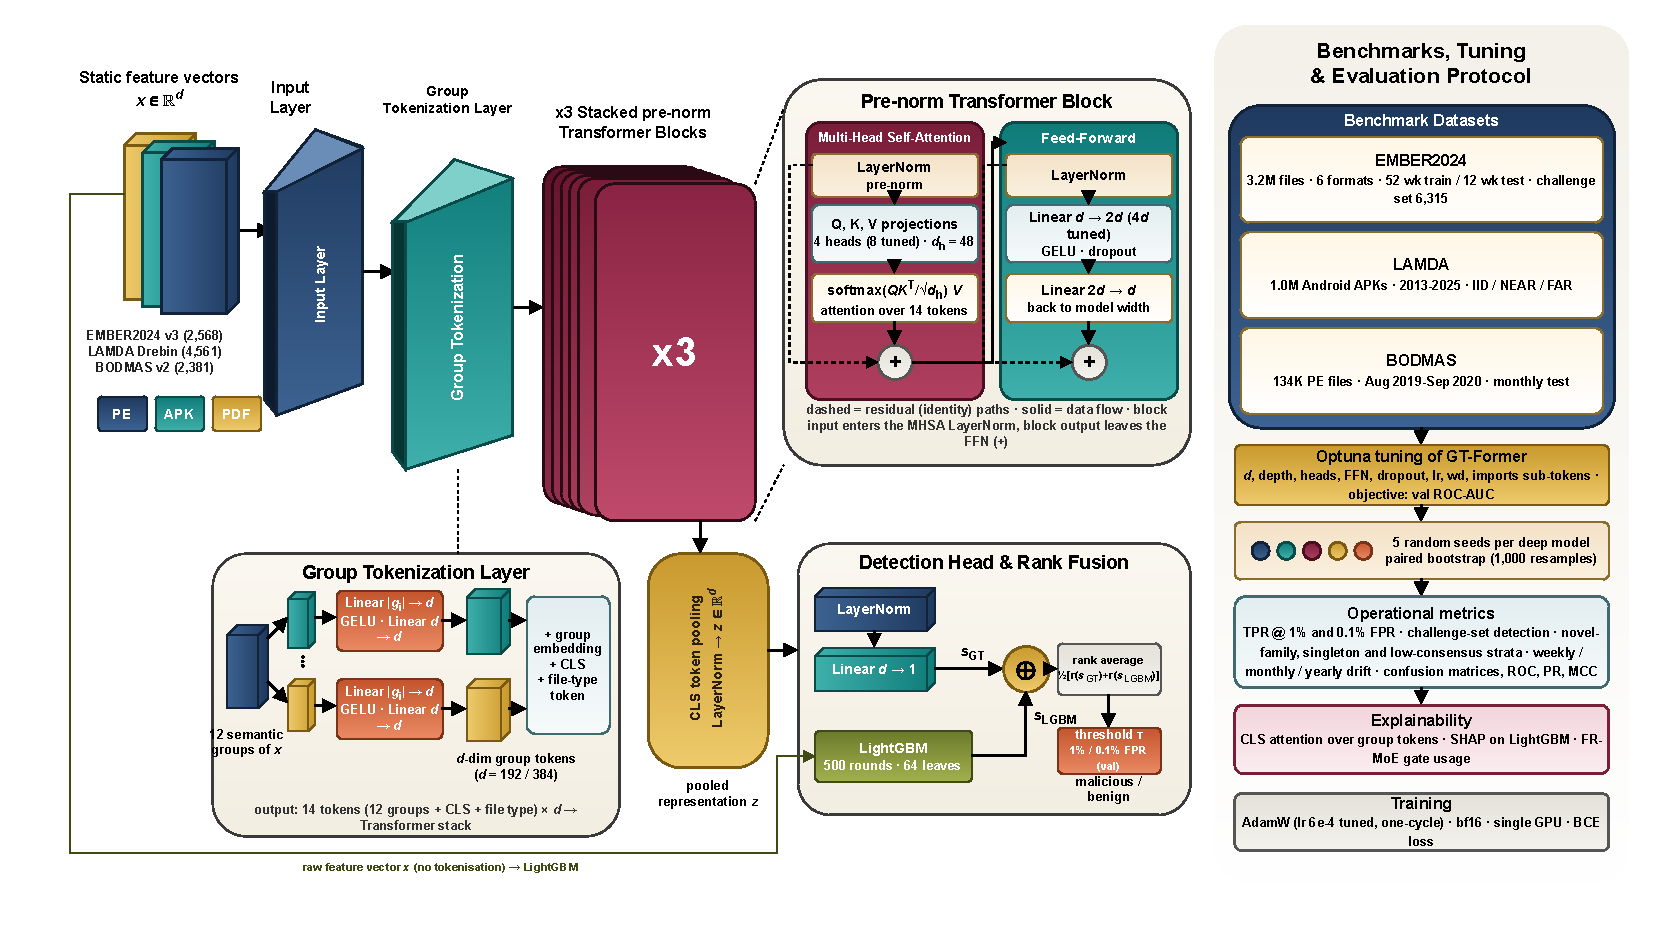
\includegraphics[width=\textwidth]{Fig1_GTFormer.pdf}
\caption{\gtf{} architecture. Static feature vectors from the three benchmarks pass through the input layer and the Group Tokenization Layer (detail, bottom left), three stacked pre-norm Transformer blocks (detail, top centre), CLS pooling and the detection head (LayerNorm, linear $d \to 1$); the detection logit is rank-fused with \lgbm{}, which receives the raw feature vector directly (bypass line), and thresholded at a fixed false-positive rate. Right: benchmarks, Optuna tuning, seeds and the evaluation protocol.}
\label{fig:gtformer}
\end{sidewaysfigure}

\paragraph{\gtf{} (Group-Token Transformer)}
Following the observation that semantically grouped features fused by attention generalise better to unseen families than a flat encoder\cite{aljarrah2026crossattention}, the feature vector is split into its semantic groups $g_1, \dots, g_G$ (EMBER: general 7, byte histogram 256, byte-entropy 256, strings 177, header 74, sections 224, imports 1,282, exports 129, data directories 34, rich header 33, Authenticode 8, pefile warnings 88; LAMDA: the ten Drebin categories). Each group is projected by a two-layer MLP to a $d$-dimensional token and summed with a learned group embedding $E_i$,
\begin{equation}
h_i = W_2\, \mathrm{GELU}(W_1 \tilde{x}_{g_i} + b_1) + b_2 + E_i, \qquad i = 1, \dots, G,
\label{eq:token}
\end{equation}
with $d = 192$ by default. On EMBER a file-type embedding token $h_t$ is added and a learnable CLS token is prepended, giving $H_0 = [\,h_{\mathrm{CLS}};\, h_t;\, h_1; \dots; h_G\,]$ with 14 tokens on EMBER and 11 on LAMDA. A three-layer pre-norm Transformer encoder\cite{vaswani2017attention} with four heads, feed-forward width 384 and dropout 0.1 processes the sequence,
\begin{equation}
H'_{\ell} = H_{\ell-1} + \mathrm{MHSA}(\LN(H_{\ell-1})), \qquad H_{\ell} = H'_{\ell} + \mathrm{FFN}(\LN(H'_{\ell})),
\label{eq:block}
\end{equation}
and the CLS output after LayerNorm is the representation $z = \LN(H_L[\mathrm{CLS}]) \in \mathbb{R}^{d}$, from which a linear head produces the logit $s_{\mathrm{GT}} = w^{\top} z + b$. The default model has 2.13\,M parameters on EMBER.

\paragraph{FR-MoE (Format-Routed Mixture of Experts, EMBER only)}
A shared trunk ($2{,}568 + 32 \to 1{,}024 \to 512$, GELU, LayerNorm) feeds six experts ($512 \to 384 \to 192$) and a shared expert; a gate conditioned on the trunk output \emph{and} the file-type embedding produces soft mixing weights. The model has 5.28\,M parameters.

\paragraph{ProtoCon-Net}
Prototype-based classification has proved effective for scarce and drifting malware families\cite{tawfik2026fewshot}. An MLP encoder (input $\to 1{,}024 \to 512 \to 192$, LayerNorm) is followed by $K = 4$ learnable prototypes per class, $\{p_{ck}\}$, and the detection logit is
\begin{equation}
s = \lse_{k}\, \frac{\cos(z, p_{1k})}{\tau} - \lse_{k}\, \frac{\cos(z, p_{0k})}{\tau}, \qquad \tau = 0.1 .
\label{eq:proto}
\end{equation}
A projection head ($192 \to 128$) receives a supervised-contrastive loss\cite{khosla2020supcon} whose positives are same-family malware pairs or benign--benign pairs ($\lambda_{\mathrm{con}} = 0.3$). The model has 3.65\,M parameters on EMBER.

\paragraph{Hyper-parameter tuning of \gtf{}}
Because a fixed default configuration is an unfair representative of an architecture, the width (128--384), depth (2--6), number of heads (4 or 8), dropout (0--0.3), learning rate ($2 \times 10^{-4}$ to $3 \times 10^{-3}$), weight decay ($10^{-6}$ to $10^{-2}$), feed-forward multiplier (2 or 4) and the number of sub-tokens for the 1,282-dimensional imports block (1, 2 or 4) of \gtf{} were tuned with Optuna\cite{akiba2019optuna} using the TPE sampler: 20 trials on a 300\,K-file, 3-epoch EMBER2024 proxy, 25 trials on LAMDA and 25 on BODMAS, with validation ROC-AUC on the time-aware validation split as the objective. The selected EMBER2024 configuration is $d = 384$, 3 layers, 8 heads, feed-forward multiplier 4, imports split into two tokens, dropout 0.12 and learning rate $6 \times 10^{-4}$ (7.9\,M parameters); LAMDA selects $d = 384$, 3 layers and 8 heads; BODMAS selects $d = 192$, 3 layers and 8 heads. All tuning and training ran on a single GPU.

\paragraph{Reference models}
We use the EMBER2024 \lgbm{} configuration (500 rounds, 64 leaves, learning rate 0.1, \texttt{is\_unbalance}), with one model per format on EMBER and one model on LAMDA, using the same validation data for early stopping; and a plain MLP with the ProtoCon-Net encoder and a linear head (3.58\,M parameters on EMBER).

\paragraph{Hybrid rank fusion}
Given the test scores of a deep model and of \lgbm{} over the same $N$ files, the fused score is the average of their normalised ranks,
\begin{equation}
s_{\mathrm{fus}} = \tfrac{1}{2}\left[ \rank(s_{\mathrm{GT}})/N + \rank(s_{\mathrm{LGBM}})/N \right],
\label{eq:fusion}
\end{equation}
so that the two models contribute equally regardless of their score scales; the fused score is then thresholded exactly like a single model.

\subsection{Training protocol}
\label{sec:training}
On EMBER the deep models are trained jointly on all formats (2,626,000 files) with format-balanced sampling (probability proportional to $1/\sqrt{n_{\mathrm{format}}}$), AdamW (learning rate $10^{-3}$ for \gtf{} and $5 \times 10^{-4}$ otherwise, one-cycle schedule, weight decay $10^{-4}$), batch size 2,048, 8 epochs, bf16 autocast and gradient clipping at 5; model selection uses ROC-AUC on the time-aware validation window (training weeks 48--51); five seeds (0--4) are run for \gtf{} (default and tuned), the MLP and FR-MoE. On LAMDA we use the same optimiser with batch size 1,024, 12 epochs and model selection on the 15\% validation split; five seeds for \gtf{} (default and tuned) and the MLP, three for \lgbm{}. On BODMAS we use batch size 512, 15 epochs and five seeds for the tuned \gtf{}. All experiments ran on one RTX A4000 Laptop GPU (8\,GB); one EMBER deep run takes 8--25 minutes, one LAMDA run 1--3 minutes and one BODMAS run under a minute; the \lgbm{} reference on BODMAS uses the \lgbm{} GPU device.

\subsection{Evaluation protocol}
\label{sec:eval}
For a false-positive budget $\alpha$, the operating threshold is the $(1-\alpha)$ quantile of the scores of benign files,
\begin{equation}
\tau_\alpha = Q_{1-\alpha}\big(\{ s_i : y_i = 0 \}\big), \qquad \mathrm{TPR}@\alpha = \frac{1}{|\{i: y_i = 1\}|} \sum_{i : y_i = 1} \mathbb{1}[s_i \ge \tau_\alpha],
\label{eq:tpr}
\end{equation}
with the benign set taken either from the test files (comparable to prior work) or from the validation files (deployment-realistic, with the realised test FPR reported). The closed-set metrics are ROC-AUC, PR-AUC and TPR at 1\% and 0.1\% FPR, reported per format on EMBER and per region and per year on LAMDA; on LAMDA we also report F1, FNR and FPR at the 0.5 threshold for comparability with Haque et al.\cite{haque2026lamda}, for single models only, since rank-averaged scores are not probabilities. Challenge-set detection on EMBER is the fraction of challenge files of a format scored above the threshold giving 1\% (or 0.1\%) FPR on the test benign files of the same format, and also above the threshold calibrated on \emph{validation} benign files. Malware is stratified into known-family, novel-family (family never seen in training malware) and no-family or singleton strata, and into a low-consensus stratum (bottom-quartile consensus on EMBER; at most six detections on LAMDA). Drift is measured as TPR at 1\% FPR per test week on EMBER and per year on LAMDA, with the threshold fixed on the IID benign files. Uncertainty is quantified with a paired bootstrap (1,000 resamples) of the difference between each model and \lgbm{} on the same files, and as mean $\pm$ standard deviation over five seeds.

All deep scores are raw logits. Probabilities saturate in fp32 and create ties at the top of the ranking, which silently destroys TPR at 0.1\% FPR; in an early run we observed 21 Win32 benign files with logit above 17 that were indistinguishable after the sigmoid.

%% ------------------------------------------------------------------------------------------------
\section{Results}
\label{sec:results}

We report the operational picture on each benchmark in turn: the reproduction of the published baseline, detection at fixed false-positive budgets on the evasive and novel-family strata, the complementarity of the deep models with gradient boosting, the ablation of the metadata-driven objectives, drift over time, seed variability, and the conventional classical metrics. Every number is computed from the released score files; confidence intervals are paired bootstraps against \lgbm{} on the same files.

\subsection{EMBER2024}
\label{sec:ember}

\subsubsection{Reproduction of the published baseline}
\label{sec:repro}
Our de-duplicated \lgbm{} models reproduce the published ROC-AUC closely: Win32 0.9982 (paper 0.9981), Win64 0.9988 (0.9989), .NET 0.9980 (0.9980), APK 0.9842 (0.9868), ELF 0.9845 (0.9933) and PDF 0.9906 (0.9912). The small deficits on ELF and PDF are consistent with our time-aware validation split (the benchmark used a random 10\% split) and with halving the number of duplicated training rows.

\subsubsection{Detection at fixed false-positive budgets}
\label{sec:ops}
Table~\ref{tab:main} gives the main comparison on the two largest formats, and Figure~\ref{fig:ember-ops} shows challenge-set detection at 1\% and 0.1\% FPR, test TPR at 0.1\% FPR and novel-family TPR for every format. Three facts stand out. First, even the strongest single model detects only 63\% of evasive Win32 malware and 58\% of evasive Win64 malware at a 1\% false-positive budget, and 40\% and 11\% respectively at 0.1\%: the challenge set is far from solved. Second, novel-family malware is detected 8 points less often than known-family malware on Win32 (89.1\% versus 97.5\% for \lgbm{}), and on the small formats the gap is much larger (ELF: 28.6\% versus 90.7\%). Third, on its own every deep model trails \lgbm{} at strict operating points, by 1.5--5 points of TPR at 0.1\% FPR on the PE formats and by 7--13 points on APK, ELF and PDF; the differences are significant in the paired bootstrap for every format (for example, Win32 tuned \gtf{} challenge detection at 1\% FPR: $-12.0$ points, CI $-13.5$ to $-10.6$). Optuna tuning narrows but does not close the gap: on Win32 it lifts \gtf{} from 87.8\% to 88.5\% TPR at 0.1\% FPR and from 33.2\% to 41.5\% challenge detection at 0.1\% FPR (seed 0), the latter above the 40.5\% of \lgbm{}.

\begin{table}[!htbp]
\centering
\scriptsize
\setlength{\tabcolsep}{2.5pt}
\caption{Main comparison on the two largest EMBER2024 formats. Thresholds for challenge detection come from test benign files. Deep models use the plain objective, seed 0 (five-seed statistics in Section~\ref{sec:seeds}). Ch.\ = challenge-set detection; Nov.\ = novel-family TPR; LC = low-consensus TPR; @1\% and @0.1\% denote the false-positive budget. Best value per column and format in bold.}
\label{tab:main}
\begin{tabular}{lccccccc}
\toprule
Model & ROC-AUC & \tprat{1} & \tprat{0.1} & Ch.@1\% & Ch.@0.1\% & Nov.@1\% & LC@1\% \\
\midrule
\multicolumn{8}{l}{\textit{Win32}} \\
\lgbm{} (benchmark) & 0.9982 & 0.9684 & 0.9002 & 0.6319 & 0.4047 & 0.8914 & 0.9095 \\
MLP & 0.9974 & 0.9540 & 0.8574 & 0.4874 & 0.3113 & 0.8811 & 0.8714 \\
\gtf{} (default) & 0.9975 & 0.9598 & 0.8775 & 0.5011 & 0.3318 & 0.8935 & 0.8856 \\
\gtf{} (Optuna-tuned) & 0.9976 & 0.9613 & 0.8852 & 0.5116 & 0.4149 & 0.8935 & 0.8900 \\
FR-MoE & 0.9973 & 0.9548 & 0.8535 & 0.4887 & 0.3234 & 0.8821 & 0.8741 \\
ProtoCon-Net & 0.9975 & 0.9555 & 0.8692 & 0.4859 & 0.3216 & 0.8842 & 0.8760 \\
Fusion: \gtf{} + \lgbm{} & 0.9984 & 0.9708 & 0.9084 & 0.6719 & 0.4121 & 0.9121 & 0.9142 \\
Fusion: tuned \gtf{} + \lgbm{} & \textbf{0.9984} & \textbf{0.9727} & \textbf{0.9098} & \textbf{0.6881} & \textbf{0.4174} & \textbf{0.9183} & \textbf{0.9160} \\
\midrule
\multicolumn{8}{l}{\textit{Win64}} \\
\lgbm{} (benchmark) & 0.9988 & 0.9807 & 0.9198 & 0.5786 & 0.1130 & 0.9649 & 0.9616 \\
MLP & 0.9978 & 0.9735 & 0.8619 & 0.5086 & 0.1020 & 0.9518 & 0.9471 \\
\gtf{} (default) & 0.9979 & 0.9733 & 0.8719 & 0.5258 & 0.1278 & 0.9535 & 0.9442 \\
\gtf{} (Optuna-tuned) & 0.9981 & 0.9762 & 0.8739 & 0.5307 & 0.1118 & 0.9567 & 0.9490 \\
Fusion: \gtf{} + \lgbm{} & 0.9987 & 0.9815 & \textbf{0.9227} & \textbf{0.5872} & \textbf{0.1388} & 0.9698 & 0.9621 \\
Fusion: tuned \gtf{} + \lgbm{} & \textbf{0.9988} & \textbf{0.9828} & 0.9203 & \textbf{0.5872} & 0.1278 & \textbf{0.9706} & \textbf{0.9626} \\
\bottomrule
\end{tabular}
\end{table}

\begin{figure}[!htbp]
\centering
\begin{minipage}[t]{0.49\textwidth}\centering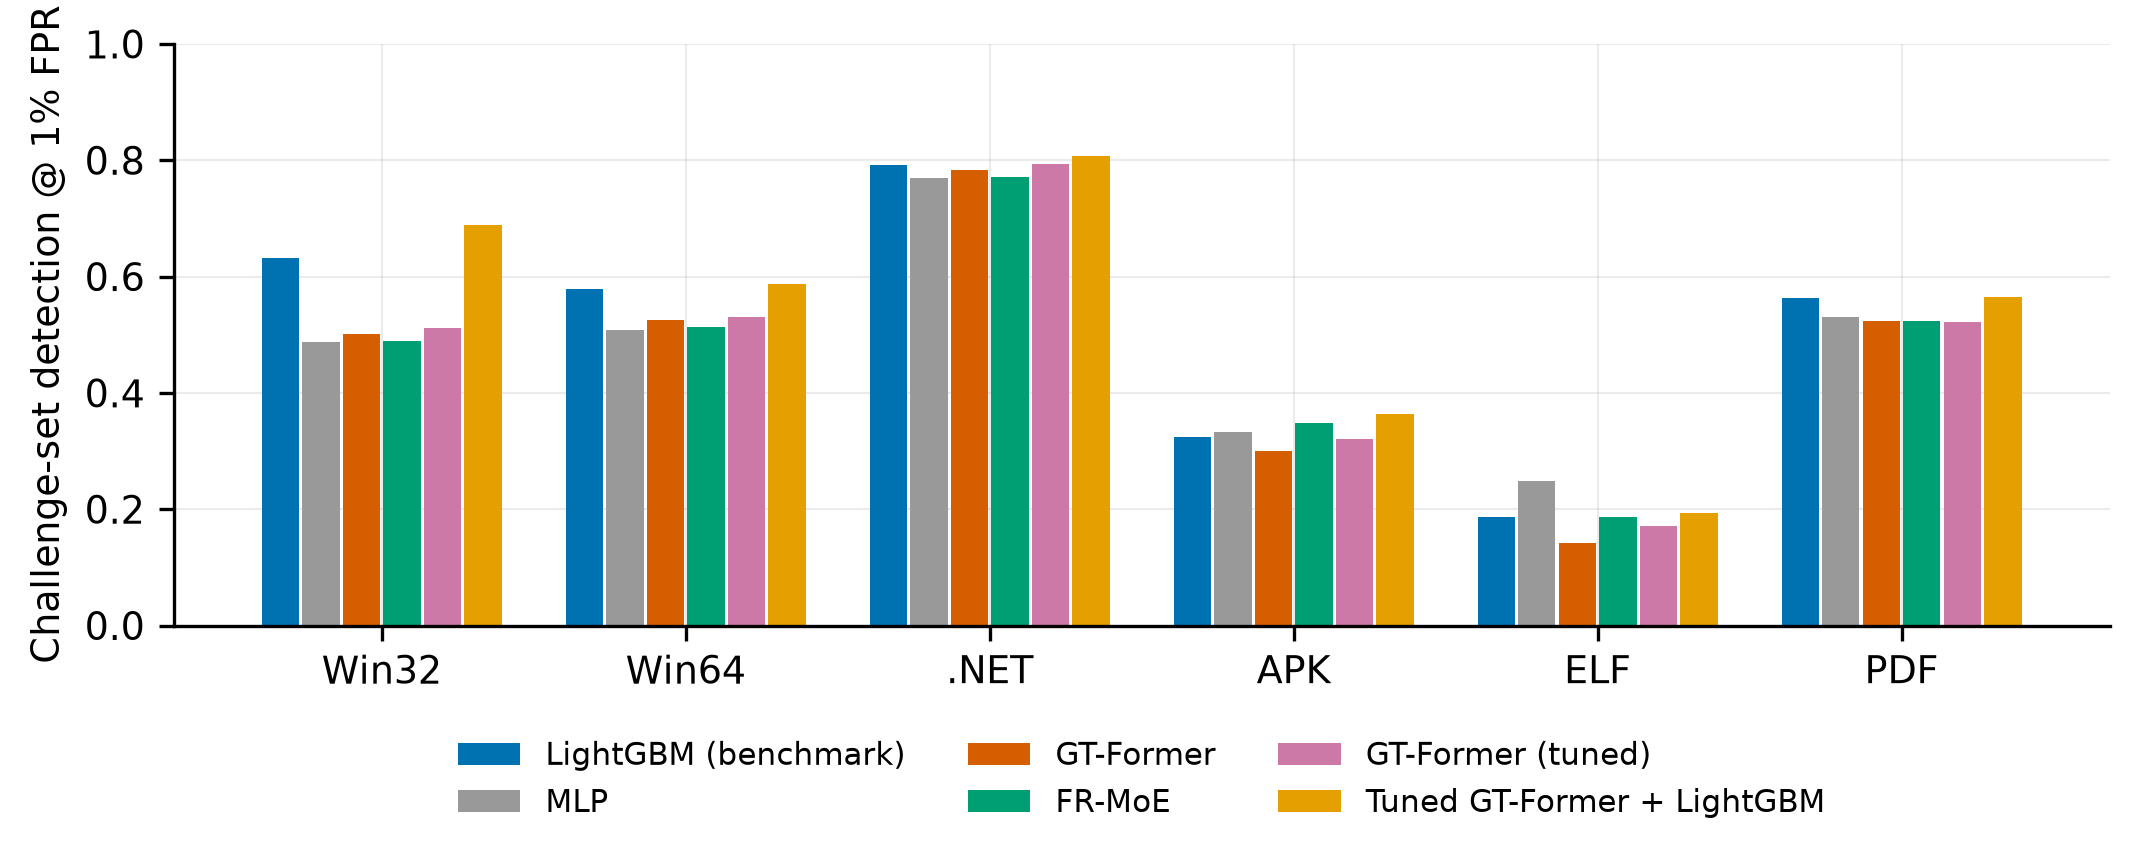
\includegraphics[width=\textwidth]{fig_challenge_1pct.png}\\ {\small (a) challenge-set detection at 1\% FPR}\end{minipage}\hfill
\begin{minipage}[t]{0.49\textwidth}\centering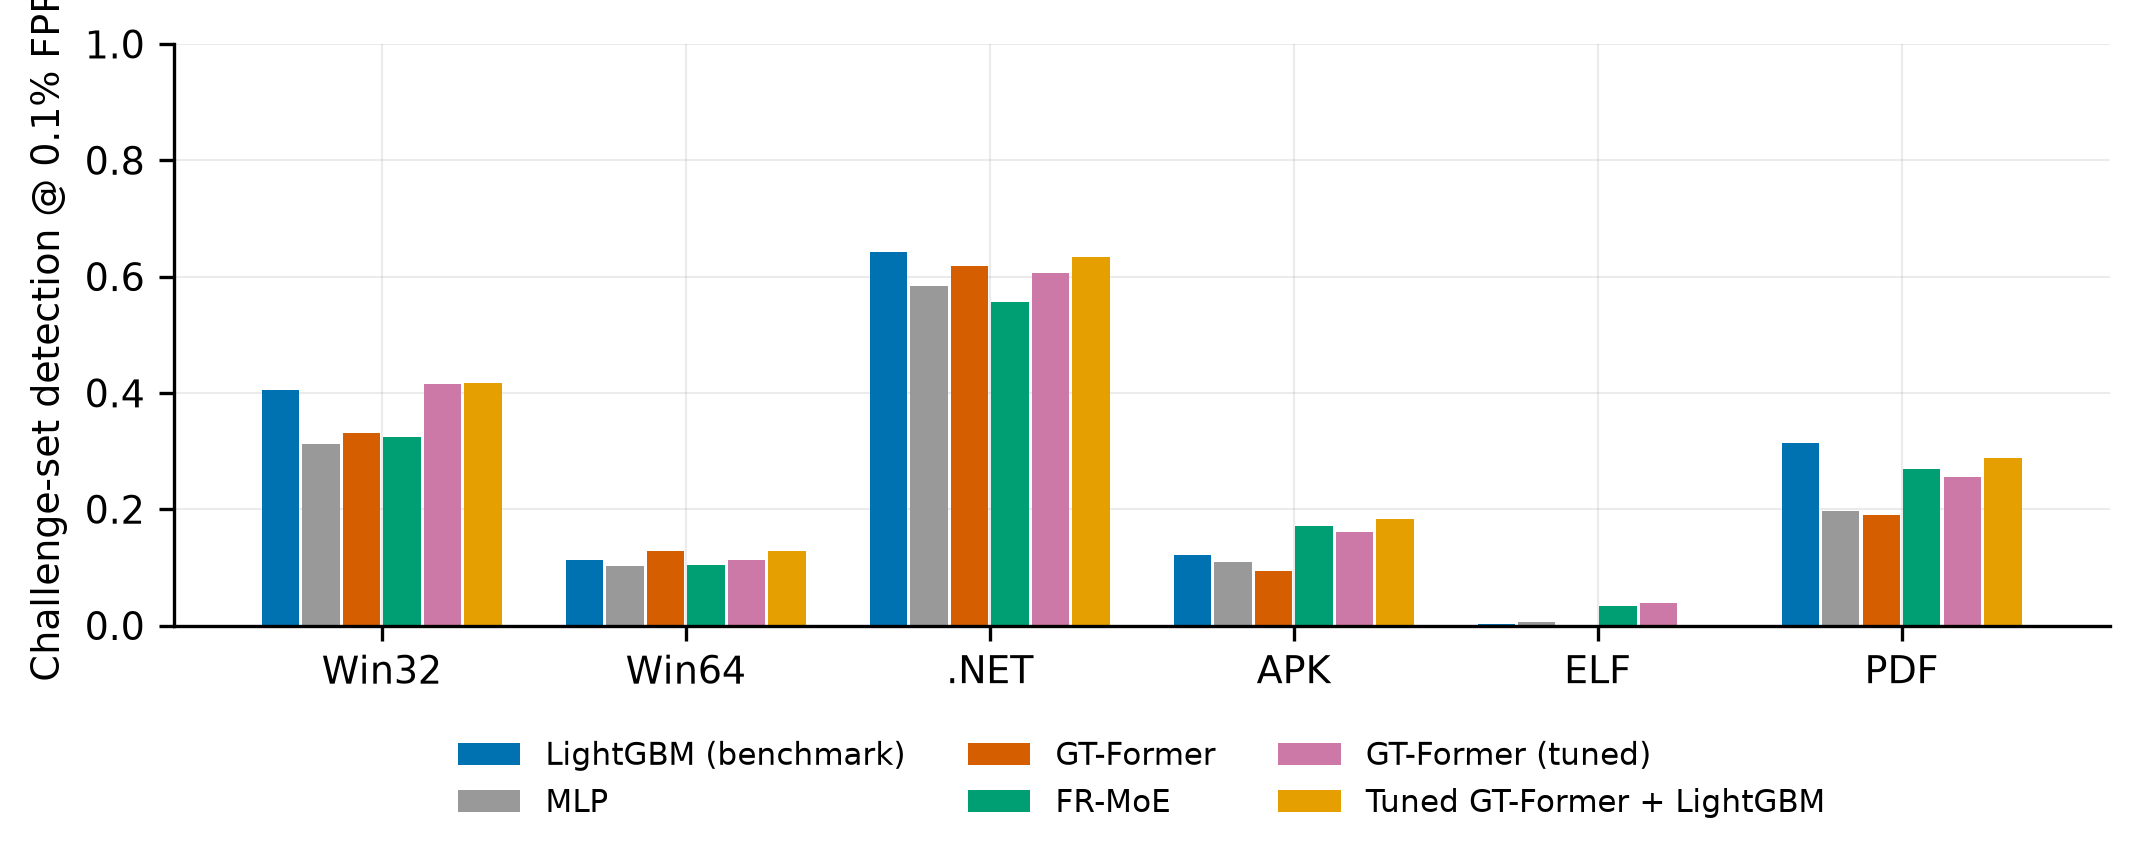
\includegraphics[width=\textwidth]{fig_challenge_01pct.png}\\ {\small (b) challenge-set detection at 0.1\% FPR}\end{minipage}\\[6pt]
\begin{minipage}[t]{0.49\textwidth}\centering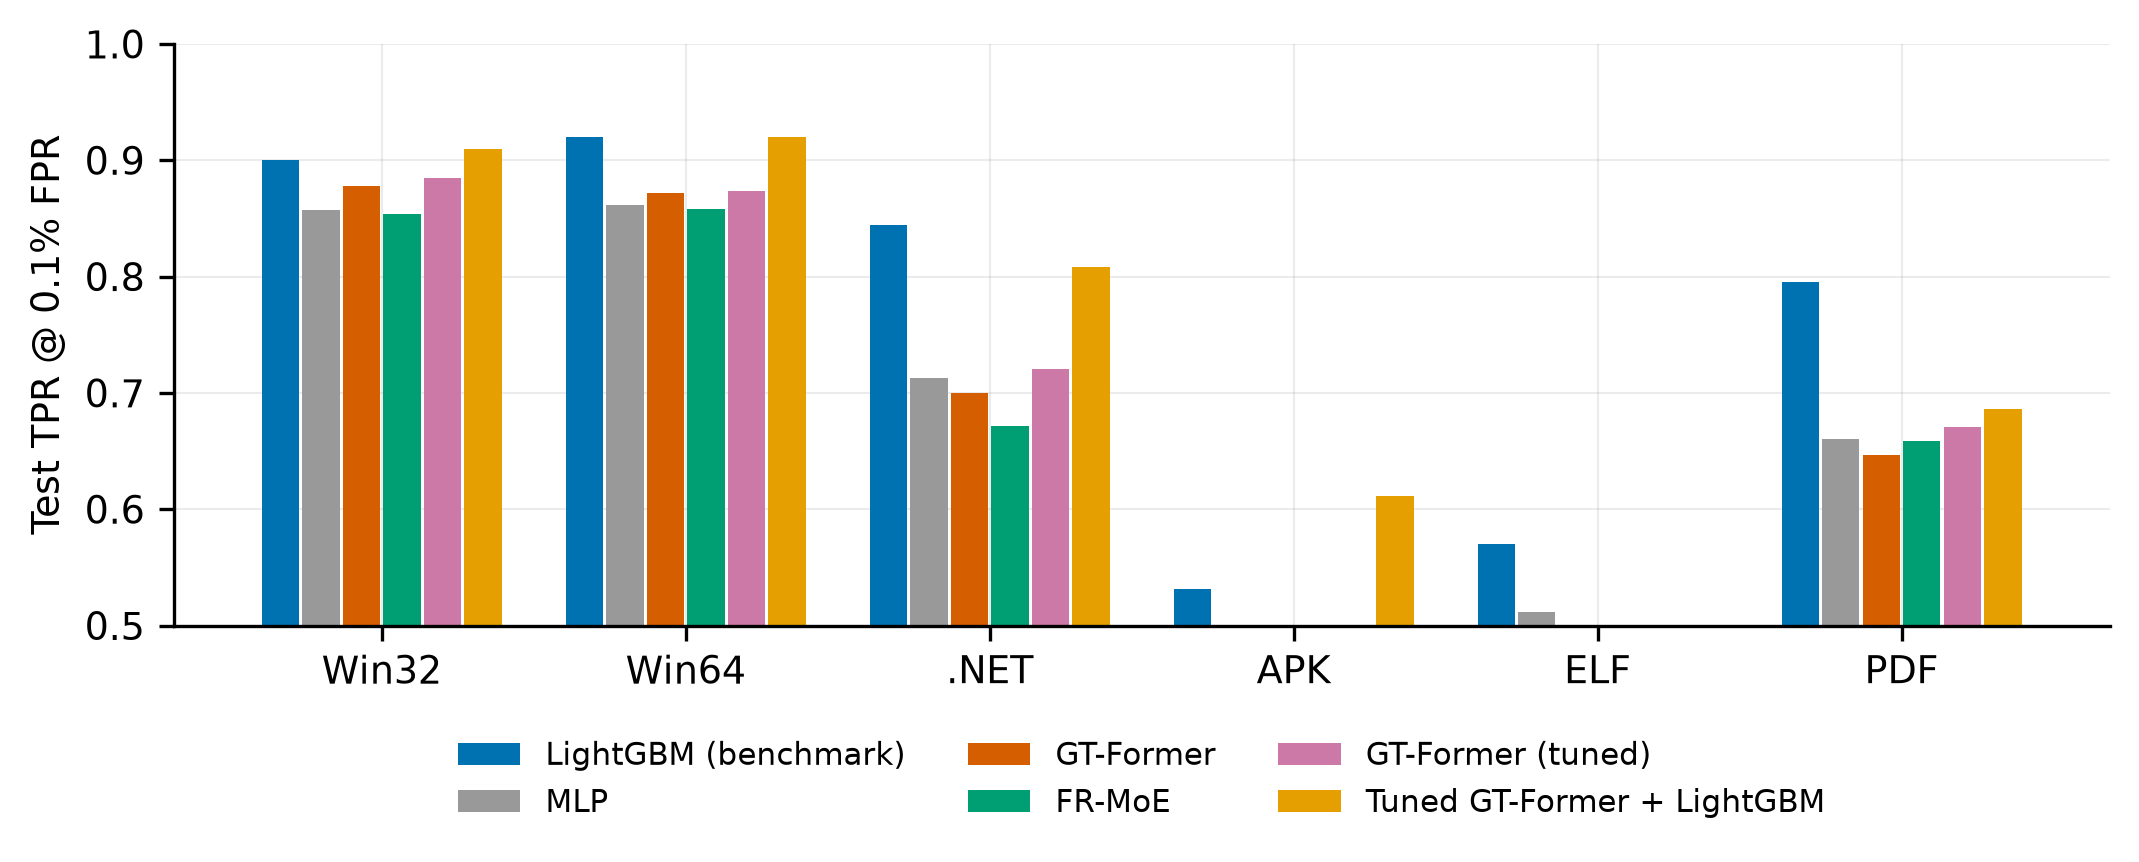
\includegraphics[width=\textwidth]{fig_test_tpr_01pct.png}\\ {\small (c) test TPR at 0.1\% FPR}\end{minipage}\hfill
\begin{minipage}[t]{0.49\textwidth}\centering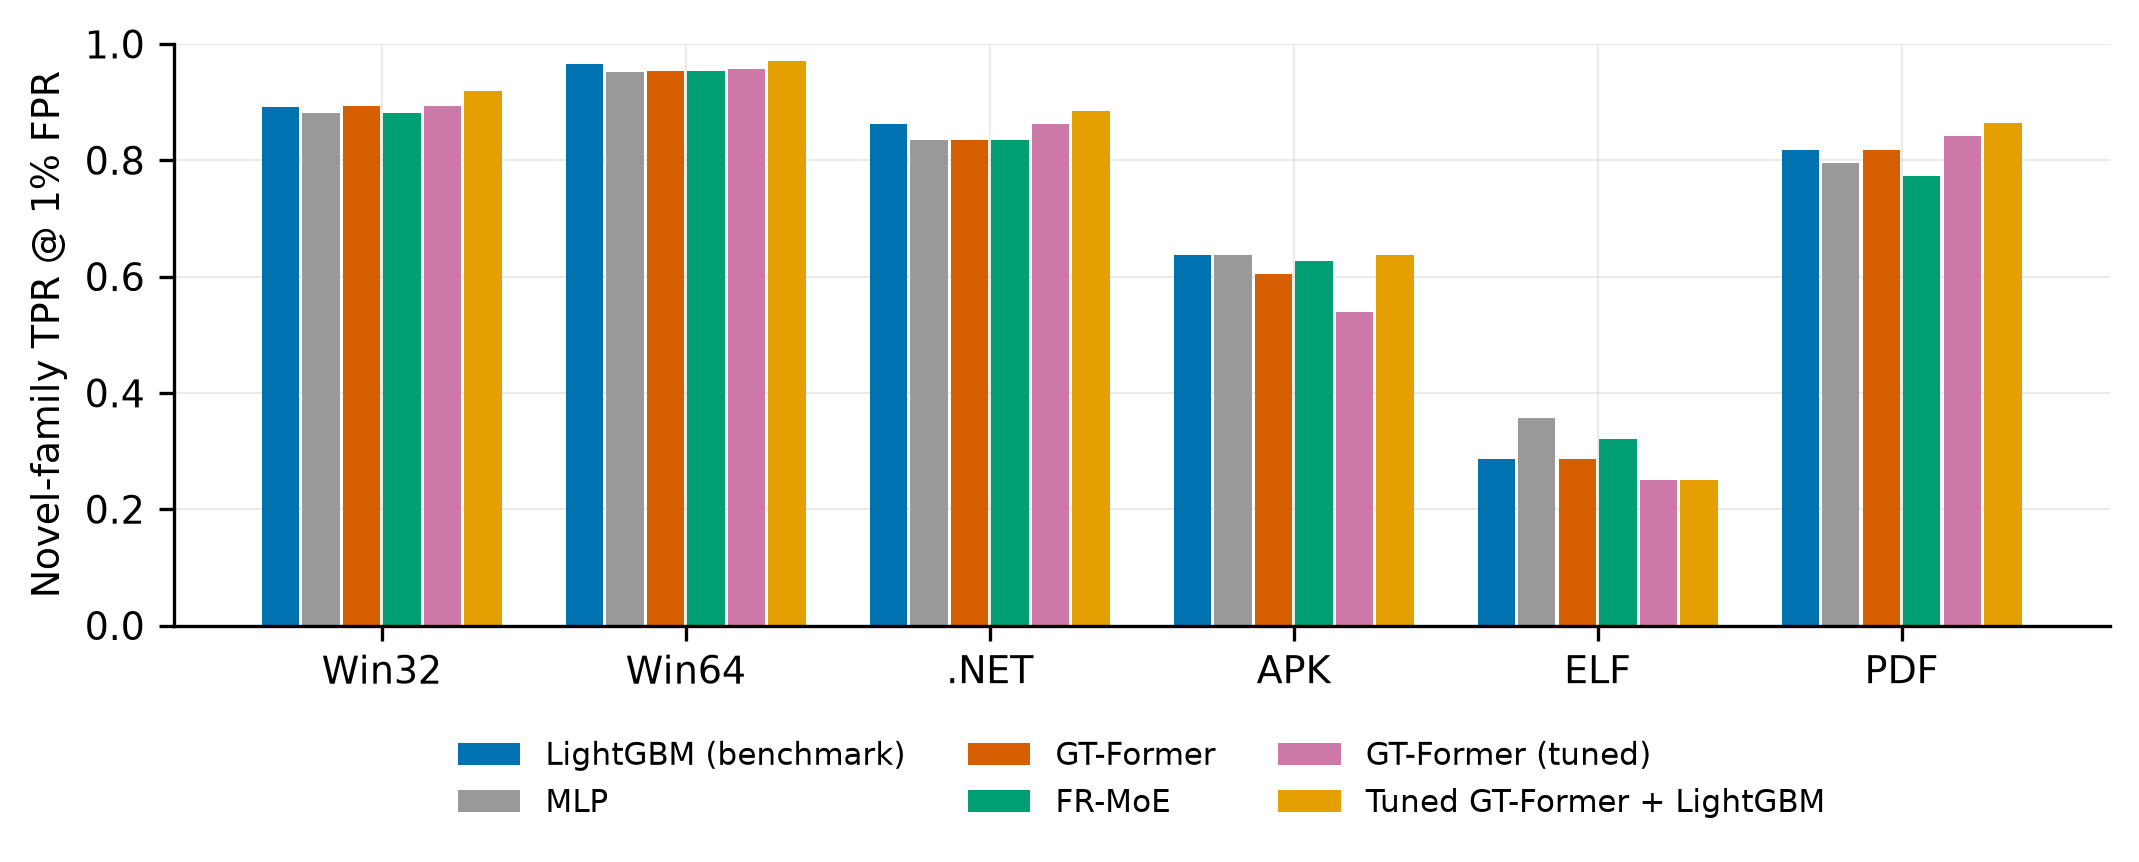
\includegraphics[width=\textwidth]{fig_novel_family.png}\\ {\small (d) novel-family TPR at 1\% FPR}\end{minipage}
\caption{EMBER2024 operational metrics per format (thresholds from test benign files) for \lgbm{}, the deep models, the default and Optuna-tuned \gtf{}, and the tuned fusion: (a) challenge-set detection at 1\% FPR, (b) challenge-set detection at 0.1\% FPR, (c) test TPR at 0.1\% FPR, (d) novel-family TPR at 1\% FPR.}
\label{fig:ember-ops}
\end{figure}

\subsubsection{Hybrid rank fusion: \gtf{} is complementary to gradient boosting}
\label{sec:fusion}
A rank average of \gtf{} and \lgbm{} scores is better than \lgbm{} alone on Win32 for every metric in Table~\ref{tab:main}, and the gains grow with the tuned \gtf{}. With the default \gtf{}, challenge detection at 1\% FPR rises from 63.2\% to 67.2\% ($+4.0$ points, 95\% CI $+3.1$ to $+4.9$) and novel-family detection from 89.1\% to 91.2\% ($+2.1$, CI $+0.8$ to $+3.4$). With the Optuna-tuned \gtf{} the same fusion reaches 68.8\% challenge detection ($+5.6$, CI $+4.7$ to $+6.6$), 91.8\% novel-family detection ($+2.7$, CI $+1.5$ to $+3.9$) and 97.3\% test TPR at 1\% FPR ($+0.4$, CI $+0.4$ to $+0.5$), with TPR at 0.1\% FPR rising from 90.0\% to 91.0\%. The tuned fusion is also significantly better than \lgbm{} on .NET challenge detection (79.3\% to 80.8\%, CI $+0.1$ to $+3.1$), on APK challenge detection (32.4\% to 36.3\%, CI $+0.8$ to $+7.4$) and APK test TPR ($+1.9$, CI $+1.6$ to $+2.2$), and on Win64 test TPR ($+0.2$, CI $+0.1$ to $+0.3$); it is significantly worse only on the two smallest PE-like formats for test TPR (.NET $-0.4$, ELF $-5.8$), where the tuned transformer itself is unstable. On the unweighted mean over the six formats the tuned fusion has the best challenge detection at 1\% and 0.1\% FPR (0.5344 and 0.2750 versus 0.5130 and 0.2664 for \lgbm{} and the default fusion the best TPR at 1\% FPR (0.9198), at two to three times the inference cost (17--30\,\textmu s versus 9\,\textmu s per file). Ensembling all three deep models with \lgbm{} is \emph{worse} than the two-model ensemble on Win32 (challenge detection at 1\% FPR 52.4\%), because the MLP and FR-MoE errors are highly correlated with each other and the average drowns the tree model.

\subsubsection{Ablation of the metadata-driven objectives}
\label{sec:ablation}
Table~\ref{tab:ablation} and Figure~\ref{fig:ablation} report the ablation of the three metadata-driven terms of Eq.~\eqref{eq:loss} as unweighted means over the six formats. For every architecture the full objective lowers TPR at 0.1\% FPR by 14--40 points and does not raise challenge detection. The validation curves tell the same story: \gtf{} reaches 0.9964 validation AUC with the plain objective, 0.9963 without the family head, 0.9952 without CAM, 0.9947 without the consensus head and 0.9941 with everything switched on. Removing the family-adversarial head alone recovers essentially all of the loss at 1\% FPR, so gradient reversal is the main culprit: forcing the encoder to forget family identity also removes information that separates malware from benign files, and the novel-family stratum does \emph{not} benefit (0.687 with gradient reversal versus 0.732 without). CAM shifts the decision boundary for low-consensus malware, but the challenge files are not the low-consensus \emph{training} files: CAM lowers TPR at strict FPR without improving challenge detection. The tree analogues behave the same way: consensus weights, family-balanced weights and their inverse control are all within $\pm 2$ points of the benchmark on every metric.

\begin{table}[!htbp]
\centering
\scriptsize
\setlength{\tabcolsep}{2.5pt}
\caption{Ablation of the metadata-driven objectives on EMBER2024, unweighted mean over the six formats. Ch.\ = challenge-set detection; Nov.\ = novel-family TPR; LC = low-consensus TPR.}
\label{tab:ablation}
\begin{tabular}{lcccccc}
\toprule
Variant & \tprat{1} & \tprat{0.1} & Ch.@1\% & Ch.@0.1\% & Nov.@1\% & LC@1\% \\
\midrule
\gtf{} plain & 0.8769 & 0.6012 & 0.4629 & 0.2268 & 0.7317 & 0.7761 \\
\gtf{} full (CAM + cons.\ head + family GRL) & 0.8187 & 0.4577 & 0.4395 & 0.2131 & 0.6860 & 0.7101 \\
\quad $-$ CAM & 0.8648 & 0.5793 & 0.4710 & 0.2155 & 0.7321 & 0.7553 \\
\quad $-$ consensus head & 0.7598 & 0.3438 & 0.4270 & 0.2348 & 0.6557 & 0.6841 \\
\quad $-$ family GRL & 0.8635 & 0.6295 & 0.4732 & 0.2263 & 0.6873 & 0.7663 \\
MLP plain & 0.8814 & 0.6821 & 0.4795 & 0.2182 & 0.7430 & 0.7857 \\
MLP full & 0.7406 & 0.3062 & 0.4491 & 0.2160 & 0.6697 & 0.7118 \\
FR-MoE plain & 0.8641 & 0.6633 & 0.4719 & 0.2430 & 0.7320 & 0.7685 \\
FR-MoE full & 0.8049 & 0.3526 & 0.4680 & 0.1051 & 0.7306 & 0.7389 \\
ProtoCon-Net plain & 0.8755 & 0.7049 & 0.4619 & 0.2308 & 0.7225 & 0.7774 \\
ProtoCon-Net full & 0.7413 & 0.3068 & 0.4277 & 0.1870 & 0.6701 & 0.6854 \\
ProtoCon-Net $-$ SupCon & 0.7493 & 0.3521 & 0.4124 & 0.2099 & 0.7180 & 0.6956 \\
\bottomrule
\end{tabular}
\end{table}

\begin{figure}[!htbp]
\centering
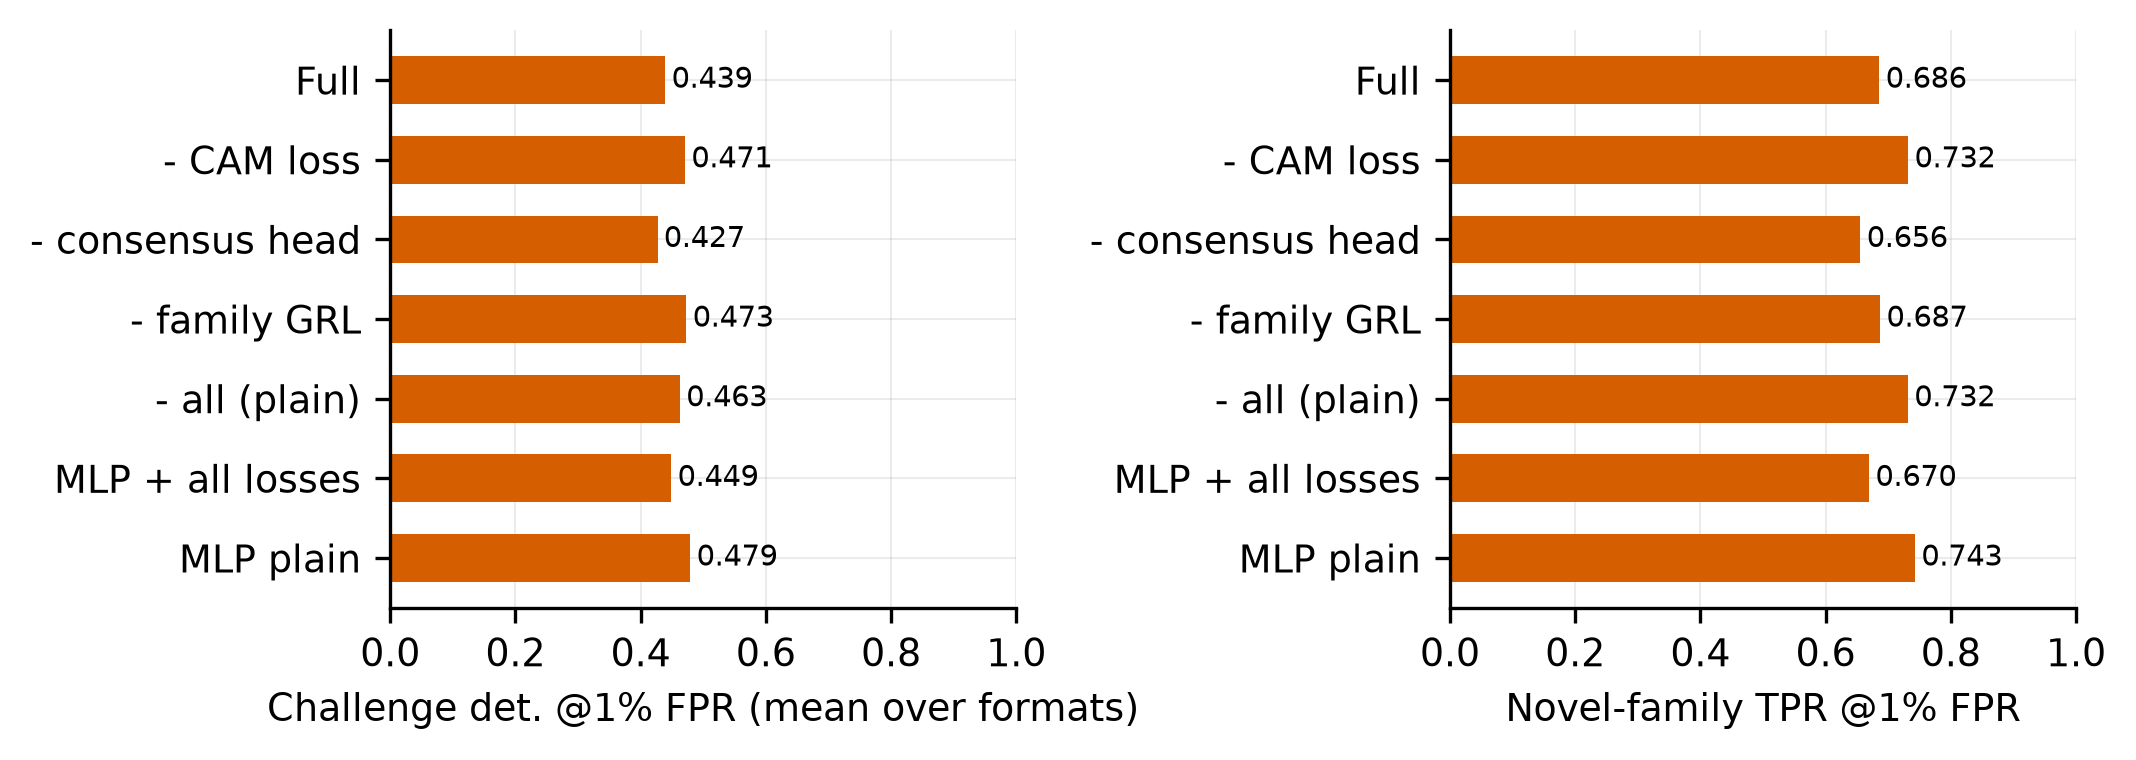
\includegraphics[width=0.8\textwidth]{fig_ablation.png}
\caption{\gtf{} component ablation (mean over the six EMBER2024 formats).}
\label{fig:ablation}
\end{figure}

\subsubsection{Drift over the twelve test weeks}
\label{sec:weekly}
Figure~\ref{fig:weekly} plots TPR at 1\% FPR per test week. It is flat on Win32, Win64 and .NET for all models (Win32 \lgbm{}: 0.973 in week 52 and 0.962 in week 63). The small formats drift: on APK all models lose 6--7 points between weeks 52 and 60 in lock-step (\lgbm{} 0.823 to 0.758), and on PDF the MLP and FR-MoE collapse to 0.63 and 0.49 in weeks 59--62 while \lgbm{} (0.91) and \gtf{} (0.80) hold up. The group-token architecture is therefore markedly more robust to the PDF benign-distribution shift than the flat encoders, though still less robust than the tree model.

\begin{figure}[!htbp]
\centering
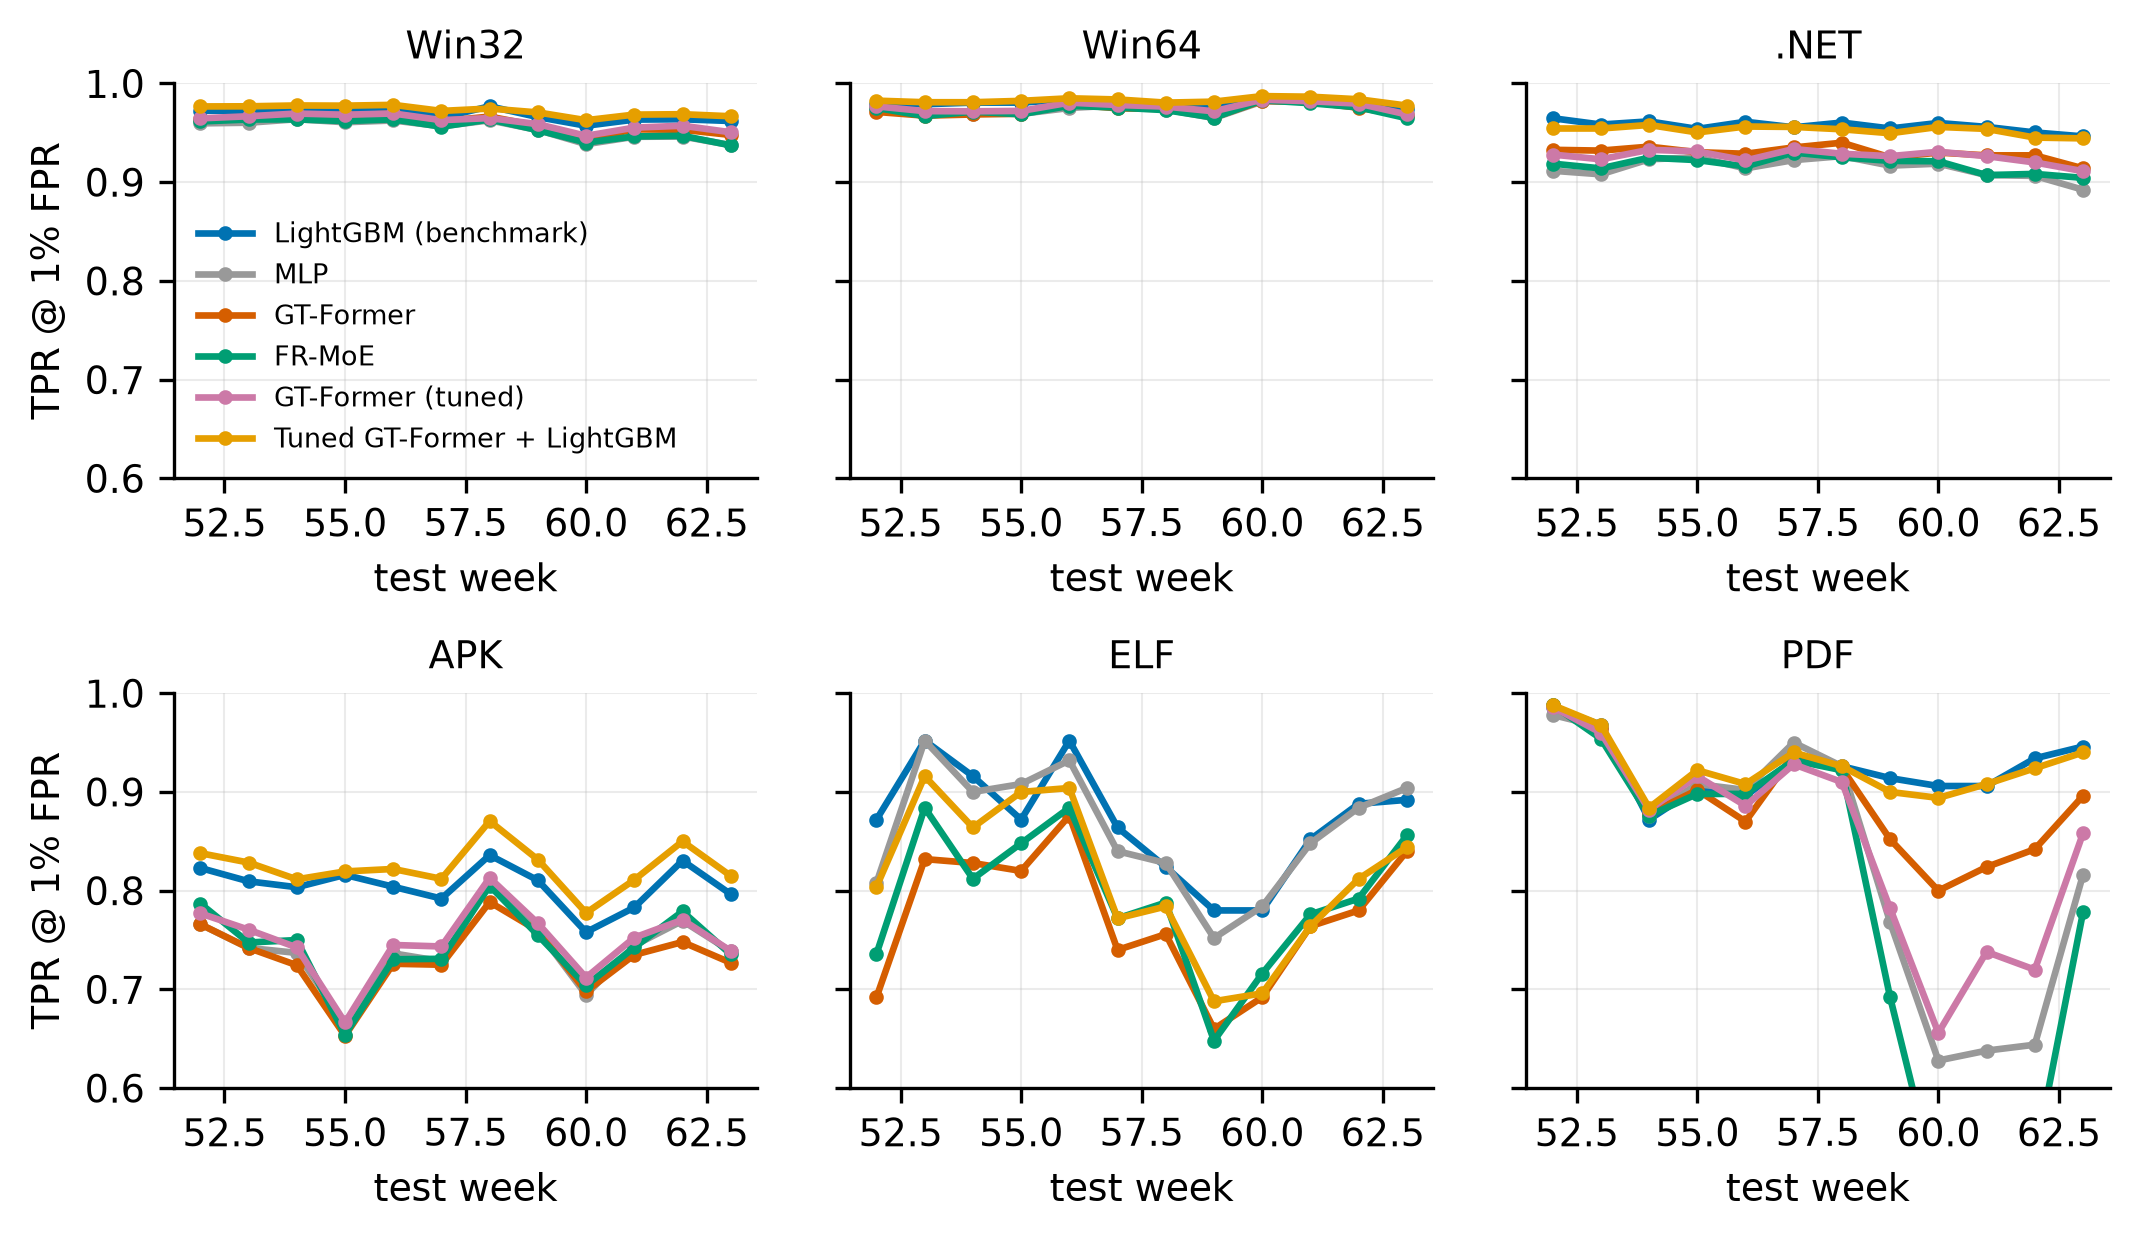
\includegraphics[width=\textwidth]{fig_weekly_drift.png}
\caption{EMBER2024: TPR at 1\% FPR per test week (weeks 52--63) and format.}
\label{fig:weekly}
\end{figure}

\subsubsection{Seed variability}
\label{sec:seeds}
Over five seeds the deep models are stable on the large formats and unstable on the smallest. On Win32 the default \gtf{} reaches TPR at 0.1\% FPR of $0.879 \pm 0.003$, challenge detection at 1\% FPR of $0.495 \pm 0.004$ and novel-family TPR of $0.891 \pm 0.004$; the tuned \gtf{} reaches $0.881 \pm 0.004$, $0.523 \pm 0.031$ and $0.892 \pm 0.003$; the MLP $0.859 \pm 0.001$, $0.487 \pm 0.003$ and $0.888 \pm 0.006$; and FR-MoE $0.857 \pm 0.004$, $0.488 \pm 0.003$ and $0.886 \pm 0.004$. On Win64 the tuned \gtf{} reaches challenge detection of $0.541 \pm 0.009$ versus $0.531 \pm 0.005$ for the default. On .NET the tuned \gtf{} reaches challenge detection of $0.800 \pm 0.011$ (\lgbm{} 0.793) and novel-family TPR of $0.844 \pm 0.016$. On ELF the TPR at 0.1\% FPR of \gtf{} is $0.14 \pm 0.14$ (default) and $0.13 \pm 0.14$ (tuned) across seeds, so the transformer is unreliable on 26,000 training files; the MLP is the most stable deep model there ($0.53 \pm 0.08$). Any claim about ELF or PDF from a single deep run should be treated with suspicion.

\subsubsection{Calibrated thresholds}
With the threshold chosen on validation benign files to give 1\% FPR, the realised FPR on the future test set is 0.74--1.30\% on the PE formats for all models, 1.8--3.3\% on ELF and 1.5--2.3\% on PDF, so benign drift on the small formats roughly doubles the false-positive budget. Challenge detection at the validation-calibrated threshold is 60.2\% for \lgbm{} and 60.9\% for the fusion on Win32.

\subsubsection{Computational cost}
Per file, inference costs 9\,\textmu s for \lgbm{} on CPU, 8\,\textmu s for the default \gtf{}, MLP or FR-MoE on GPU, 20\,\textmu s for the tuned \gtf{} (7.9\,M parameters) and 17--30\,\textmu s for the two-model ensembles. Training \lgbm{} on all formats takes 43 minutes; the default \gtf{} trains in 9 minutes and the tuned one in 22 minutes on a laptop GPU; the Optuna study cost 20 proxy trials of about one minute each.

\subsubsection{Classical metrics, confusion matrices and curves}
\label{sec:classical}
For readers who prefer the conventional view, Tables~\ref{tab:cls-ember}--\ref{tab:cls-bodmas} report the derived classical metrics (accuracy, balanced accuracy, precision, recall, specificity, FPR, F1 and Matthews correlation coefficient) for the reference \lgbm{}, the MLP, the Optuna-tuned \gtf{} and the fusion, on every benchmark and format. The operating point is the deployment-realistic one: the score threshold that yields 1\% FPR on the \emph{validation} benign files, applied unchanged to the future test data, so that the realised FPR is what a deployment would see. Figures~\ref{fig:curves-win32}--\ref{fig:curves-pdf} give, for each EMBER2024 format, the confusion matrices at this threshold and the ROC curves (logarithmic FPR axis) and precision--recall curves on the test set and on the challenge set; the vertical dotted lines in the ROC panels mark the 1\% and 0.1\% FPR operating points. Three observations complement the operational analysis. First, at the calibrated 1\% threshold the realised FPR stays at 0.8--0.9\% on Win32 and Win64 and at 1.2--1.3\% on .NET for all models, so the calibration transfers to the future test weeks on the large PE formats, whereas on the small formats it drifts to 1.7--3.3\%. Second, accuracy and F1 hide the differences that matter: on Win32 the fusion improves accuracy over \lgbm{} by only 0.17 points (0.9786 to 0.9803) and MCC by 0.003 (0.9575 to 0.9608), yet it recovers 494 additional malware files (5,534 versus 6,028 false negatives) with 109 fewer false positives; on the challenge set mixed with test benign files the F1 of the fusion is 0.584 versus 0.568 and its MCC 0.577 versus 0.561. Third, under strong drift the classical metrics collapse for every model: on LAMDA FAR the recall at the calibrated threshold is 0.23 for \lgbm{} and 0.25 for the MLP with precision above 0.97, so the detectors are conservative rather than noisy, and the rank fusion keeps the FPR at 0.12\% while lifting the AUC to 0.916.

\begin{table}[!htbp]
\centering
\scriptsize
\setlength{\tabcolsep}{2.5pt}
\caption{EMBER2024 classical metrics at the validation-calibrated 1\% FPR threshold. Fusion = rank fusion of the tuned \gtf{} and \lgbm{}. The Win32 chall.\ rows mix the challenge files with the Win32 test benign files.}
\label{tab:cls-ember}
\begin{tabular}{llcccccccccc}
\toprule
Subset & Model & Acc. & Bal.\ acc. & Prec. & Recall & Spec. & FPR & F1 & MCC & ROC-AUC & PR-AUC \\
\midrule
Win32 & \lgbm{} & 0.9786 & 0.9786 & 0.9905 & 0.9665 & 0.9907 & 0.0093 & 0.9784 & 0.9575 & 0.9982 & 0.9983 \\
Win32 & MLP & 0.9696 & 0.9696 & 0.9914 & 0.9474 & 0.9917 & 0.0083 & 0.9689 & 0.9401 & 0.9974 & 0.9976 \\
Win32 & \gtf{} (tuned) & 0.9738 & 0.9738 & 0.9911 & 0.9561 & 0.9914 & 0.0086 & 0.9733 & 0.9482 & 0.9976 & 0.9979 \\
Win32 & Fusion & 0.9803 & 0.9803 & 0.9911 & 0.9693 & 0.9913 & 0.0087 & 0.9801 & 0.9608 & 0.9984 & 0.9985 \\
Win32 chall. & \lgbm{} & 0.9839 & 0.7963 & 0.5377 & 0.6019 & 0.9907 & 0.0093 & 0.5680 & 0.5607 & 0.9671 & 0.6441 \\
Win32 chall. & MLP & 0.9828 & 0.7362 & 0.5107 & 0.4806 & 0.9917 & 0.0083 & 0.4952 & 0.4867 & 0.9716 & 0.5590 \\
Win32 chall. & \gtf{} (tuned) & 0.9827 & 0.7446 & 0.5102 & 0.4977 & 0.9914 & 0.0086 & 0.5038 & 0.4951 & 0.9754 & 0.6391 \\
Win32 chall. & Fusion & 0.9847 & 0.8016 & 0.5584 & 0.6118 & 0.9913 & 0.0087 & 0.5839 & 0.5767 & 0.9752 & 0.6697 \\
Win64 & \lgbm{} & 0.9843 & 0.9843 & 0.9924 & 0.9759 & 0.9926 & 0.0074 & 0.9841 & 0.9686 & 0.9988 & 0.9989 \\
Win64 & MLP & 0.9810 & 0.9810 & 0.9908 & 0.9711 & 0.9909 & 0.0091 & 0.9809 & 0.9623 & 0.9978 & 0.9981 \\
Win64 & \gtf{} (tuned) & 0.9826 & 0.9826 & 0.9906 & 0.9744 & 0.9907 & 0.0093 & 0.9824 & 0.9653 & 0.9981 & 0.9983 \\
Win64 & Fusion & 0.9862 & 0.9862 & 0.9906 & 0.9817 & 0.9907 & 0.0093 & 0.9861 & 0.9725 & 0.9988 & 0.9990 \\
.NET & \lgbm{} & 0.9758 & 0.9758 & 0.9881 & 0.9633 & 0.9883 & 0.0117 & 0.9755 & 0.9519 & 0.9980 & 0.9980 \\
.NET & MLP & 0.9603 & 0.9604 & 0.9863 & 0.9337 & 0.9870 & 0.0130 & 0.9593 & 0.9220 & 0.9962 & 0.9962 \\
.NET & \gtf{} (tuned) & 0.9658 & 0.9658 & 0.9865 & 0.9446 & 0.9871 & 0.0129 & 0.9651 & 0.9325 & 0.9966 & 0.9964 \\
.NET & Fusion & 0.9748 & 0.9748 & 0.9869 & 0.9623 & 0.9872 & 0.0128 & 0.9745 & 0.9498 & 0.9978 & 0.9979 \\
APK & \lgbm{} & 0.8900 & 0.8900 & 0.9894 & 0.7884 & 0.9915 & 0.0085 & 0.8775 & 0.7966 & 0.9842 & 0.9854 \\
APK & MLP & 0.8602 & 0.8602 & 0.9879 & 0.7295 & 0.9910 & 0.0090 & 0.8392 & 0.7465 & 0.9771 & 0.9790 \\
APK & \gtf{} (tuned) & 0.8603 & 0.8603 & 0.9885 & 0.7291 & 0.9915 & 0.0085 & 0.8392 & 0.7468 & 0.9774 & 0.9795 \\
APK & Fusion & 0.8998 & 0.8998 & 0.9901 & 0.8077 & 0.9919 & 0.0081 & 0.8896 & 0.8135 & 0.9855 & 0.9868 \\
ELF & \lgbm{} & 0.9566 & 0.9566 & 0.9810 & 0.9313 & 0.9819 & 0.0181 & 0.9555 & 0.9144 & 0.9845 & 0.9874 \\
ELF & MLP & 0.9486 & 0.9486 & 0.9661 & 0.9300 & 0.9672 & 0.0328 & 0.9477 & 0.8978 & 0.9881 & 0.9893 \\
ELF & \gtf{} (tuned) & 0.9546 & 0.9546 & 0.9766 & 0.9317 & 0.9776 & 0.0224 & 0.9536 & 0.9101 & 0.9816 & 0.9757 \\
ELF & Fusion & 0.9594 & 0.9595 & 0.9745 & 0.9437 & 0.9752 & 0.0248 & 0.9588 & 0.9193 & 0.9859 & 0.9860 \\
PDF & \lgbm{} & 0.9608 & 0.9608 & 0.9764 & 0.9445 & 0.9772 & 0.0228 & 0.9602 & 0.9222 & 0.9906 & 0.9927 \\
PDF & MLP & 0.9472 & 0.9472 & 0.9817 & 0.9113 & 0.9830 & 0.0170 & 0.9452 & 0.8966 & 0.9834 & 0.9871 \\
PDF & \gtf{} (tuned) & 0.9530 & 0.9530 & 0.9740 & 0.9308 & 0.9752 & 0.0248 & 0.9519 & 0.9069 & 0.9752 & 0.9822 \\
PDF & Fusion & 0.9639 & 0.9639 & 0.9761 & 0.9512 & 0.9767 & 0.0233 & 0.9635 & 0.9281 & 0.9865 & 0.9898 \\
\bottomrule
\end{tabular}
\end{table}

\curvefig{fig_confusion_Win32.png}{fig_roc_pr_Win32_test.png}{fig_roc_pr_Win32_challenge.png}{Win32}{fig:curves-win32}
\curvefig{fig_confusion_Win64.png}{fig_roc_pr_Win64_test.png}{fig_roc_pr_Win64_challenge.png}{Win64}{fig:curves-win64}
\curvefig{fig_confusion_Dot_Net.png}{fig_roc_pr_Dot_Net_test.png}{fig_roc_pr_Dot_Net_challenge.png}{.NET}{fig:curves-dotnet}
\curvefig{fig_confusion_APK.png}{fig_roc_pr_APK_test.png}{fig_roc_pr_APK_challenge.png}{APK}{fig:curves-apk}
\curvefig{fig_confusion_ELF.png}{fig_roc_pr_ELF_test.png}{fig_roc_pr_ELF_challenge.png}{ELF}{fig:curves-elf}
\curvefig{fig_confusion_PDF.png}{fig_roc_pr_PDF_test.png}{fig_roc_pr_PDF_challenge.png}{PDF}{fig:curves-pdf}


%% ------------------------------------------------------------------------------------------------
\subsection{LAMDA}
\label{sec:lamda}

\subsubsection{Reproduction of the benchmark protocol}
Our \lgbm{} reproduces the IID numbers of the LAMDA paper exactly (F1 97.47\% versus $97.49 \pm 0.17$; FNR 2.2\%; FPR 2.4\%) and lands within its reported variance on the drift regions (NEAR F1 73.1\% versus $59.5 \pm 28.2$; FAR 58.7\% versus $47.2 \pm 27.3$; the paper's standard deviations are large because they average over years). The AUC picture is the same: 0.9963 on IID, 0.830 on NEAR and 0.886 on FAR.

\subsubsection{Operational metrics under drift}
\label{sec:lamda-ops}
Table~\ref{tab:lamda} reports the single models and the rank ensembles per region, and Figures~\ref{fig:lamda-drift} and \ref{fig:lamda-regions} show the year-by-year and region-level views. Three findings mirror EMBER2024 and one does not. First, in distribution and in the near future \lgbm{} is the best single model (NEAR TPR at 1\% FPR 52.1\% versus 39.9\% for the MLP, CI for the difference $-12.6$ to $-12.0$). Second, the evasive strata are where everything fails: singleton and low-consensus malware are detected at 30\% or less by every single model on NEAR and FAR. Third, the metadata-driven objectives hurt again: the full \gtf{} loses 5.7 points of NEAR TPR at 1\% FPR relative to the plain model (0.191 versus 0.248) and 6.4 points on FAR, and the full MLP loses 3.6 points on NEAR and 8.0 on FAR. The finding that does \emph{not} transfer is the ranking of deep models. On LAMDA the flat MLP is the most drift-robust single model on the FAR years (TPR at 1\% FPR 49.1\% versus 40.5\% for \lgbm{}, $+8.6$ points, CI $+8.4$ to $+8.8$; singleton detection 48.9\% versus 34.6\%), whereas \gtf{} is the weakest even after Optuna tuning (FAR TPR at 1\% FPR $0.28 \pm 0.03$ default and $0.29 \pm 0.05$ tuned over five seeds; MLP $0.49 \pm 0.03$; \lgbm{} has no seed variance at this configuration). Tuning raised the validation AUC of the transformer from 0.9941 to 0.9947 and its NEAR TPR from 24.8\% to 29.3\%, but the gap to the MLP remains 20 points. Tokenising 4,561 binary indicator features by Drebin category discards the fine-grained co-occurrence information that the flat encoder exploits, whereas on EMBER version-3 features the groups are semantically coherent numeric blocks. The choice of architecture must follow the semantics of the feature vector.

\begin{table}[!htbp]
\centering
\scriptsize
\setlength{\tabcolsep}{2.5pt}
\caption{LAMDA: single models (seed 0) and rank ensembles. TPR at 1\% FPR uses the threshold that gives 1\% FPR on the benign files of the same region; strata as in Section~\ref{sec:eval} (Known = known-family TPR; Nov.\ = novel-family TPR, only 13 such files exist on IID; Single.\ = singleton TPR; LC = low-consensus TPR). F1 is at threshold 0.5 and is only meaningful for single models. Best value per column in bold.}
\label{tab:lamda}
\begin{tabular}{llcccccccc}
\toprule
Model & Region & ROC-AUC & F1@0.5 & \tprat{1} & \tprat{0.1} & Known@1\% & Nov.@1\% & Single.@1\% & LC@1\% \\
\midrule
\lgbm{} & IID & 0.9963 & 0.9747 & 0.9364 & 0.6824 & 0.9469 & 0.1538 & 0.7900 & 0.8957 \\
\lgbm{} & NEAR & 0.8296 & 0.7308 & 0.5213 & 0.2678 & 0.6080 & 0.3097 & 0.3057 & 0.2851 \\
\lgbm{} & FAR & 0.8855 & 0.5869 & 0.4053 & 0.1287 & 0.5808 & 0.2950 & 0.3460 & 0.2633 \\
MLP & IID & 0.9954 & 0.9697 & 0.9272 & 0.6420 & 0.9400 & 0.1538 & 0.7425 & 0.8683 \\
MLP & NEAR & 0.8431 & 0.6746 & 0.3986 & 0.1131 & 0.4803 & 0.1979 & 0.1953 & 0.1609 \\
MLP & FAR & \textbf{0.9184} & 0.5855 & \textbf{0.4914} & \textbf{0.1777} & 0.5804 & 0.2756 & \textbf{0.4890} & \textbf{0.3614} \\
\gtf{} (default) & IID & 0.9947 & 0.9682 & 0.9269 & 0.5860 & 0.9376 & 0.0769 & 0.7800 & 0.8787 \\
\gtf{} (default) & NEAR & 0.8381 & 0.6558 & 0.2480 & 0.1159 & 0.3139 & 0.0899 & 0.0834 & 0.0623 \\
\gtf{} (default) & FAR & 0.8686 & 0.3536 & 0.2304 & 0.0752 & 0.5398 & 0.1887 & 0.0995 & 0.0881 \\
\gtf{} (tuned) & IID & 0.9953 & 0.9709 & 0.9271 & 0.6665 & 0.9380 & 0.1538 & 0.7775 & 0.8796 \\
\gtf{} (tuned) & NEAR & 0.8554 & 0.6595 & 0.2927 & 0.0742 & 0.3610 & 0.1137 & 0.1044 & 0.0855 \\
\gtf{} (tuned) & FAR & 0.8708 & 0.3521 & 0.2449 & 0.0749 & 0.5486 & 0.1985 & 0.1178 & 0.1065 \\
ProtoCon-Net & IID & 0.9951 & 0.9714 & 0.9110 & 0.5907 & 0.9242 & 0.1538 & 0.7200 & 0.8530 \\
ProtoCon-Net & NEAR & 0.8356 & 0.6663 & 0.3685 & 0.1203 & 0.4472 & 0.1850 & 0.1701 & 0.1393 \\
ProtoCon-Net & FAR & 0.9109 & 0.5930 & 0.4804 & 0.1749 & 0.5629 & 0.2482 & 0.4837 & 0.3589 \\
Fusion: MLP + \lgbm{} & IID & 0.9964 & -- & \textbf{0.9436} & 0.6793 & 0.9533 & 0.1538 & 0.8100 & 0.9011 \\
Fusion: MLP + \lgbm{} & NEAR & 0.8417 & -- & 0.4844 & \textbf{0.2825} & 0.5814 & 0.2761 & 0.2349 & 0.2198 \\
Fusion: MLP + \lgbm{} & FAR & 0.9163 & -- & \textbf{0.5436} & \textbf{0.2106} & \textbf{0.6400} & \textbf{0.3586} & \textbf{0.5326} & \textbf{0.4041} \\
\bottomrule
\end{tabular}
\end{table}

\begin{table}[!htbp]
\centering
\scriptsize
\setlength{\tabcolsep}{2.5pt}
\caption{LAMDA classical metrics at the validation-calibrated 1\% FPR threshold. Fusion = rank fusion of the MLP and \lgbm{}.}
\label{tab:cls-lamda}
\begin{tabular}{llcccccccccc}
\toprule
Region & Model & Acc. & Bal.\ acc. & Prec. & Recall & Spec. & FPR & F1 & MCC & ROC-AUC & PR-AUC \\
\midrule
IID & \lgbm{} & 0.9660 & 0.9637 & 0.9870 & 0.9378 & 0.9896 & 0.0104 & 0.9618 & 0.9322 & 0.9963 & 0.9959 \\
IID & MLP & 0.9604 & 0.9575 & 0.9885 & 0.9239 & 0.9910 & 0.0090 & 0.9551 & 0.9214 & 0.9954 & 0.9950 \\
IID & \gtf{} (tuned) & 0.9593 & 0.9563 & 0.9880 & 0.9221 & 0.9906 & 0.0094 & 0.9539 & 0.9193 & 0.9953 & 0.9947 \\
IID & Fusion & 0.9698 & 0.9679 & 0.9874 & 0.9460 & 0.9899 & 0.0101 & 0.9663 & 0.9397 & 0.9964 & 0.9961 \\
NEAR & \lgbm{} & 0.8196 & 0.7206 & 0.9738 & 0.4468 & 0.9944 & 0.0056 & 0.6126 & 0.5817 & 0.8296 & 0.8275 \\
NEAR & MLP & 0.8033 & 0.6978 & 0.9484 & 0.4059 & 0.9897 & 0.0103 & 0.5685 & 0.5369 & 0.8431 & 0.7981 \\
NEAR & \gtf{} (tuned) & 0.7844 & 0.6697 & 0.9263 & 0.3525 & 0.9869 & 0.0131 & 0.5106 & 0.4842 & 0.8554 & 0.7955 \\
NEAR & Fusion & 0.8119 & 0.7088 & 0.9693 & 0.4240 & 0.9937 & 0.0063 & 0.5899 & 0.5618 & 0.8417 & 0.8242 \\
FAR & \lgbm{} & 0.7286 & 0.6118 & 0.9722 & 0.2270 & 0.9965 & 0.0035 & 0.3681 & 0.3897 & 0.8855 & 0.8571 \\
FAR & MLP & 0.7372 & 0.6235 & 0.9848 & 0.2491 & 0.9980 & 0.0020 & 0.3976 & 0.4153 & 0.9184 & 0.8883 \\
FAR & \gtf{} (tuned) & 0.6992 & 0.5697 & 0.9551 & 0.1431 & 0.9964 & 0.0036 & 0.2488 & 0.2988 & 0.8708 & 0.8141 \\
FAR & Fusion & 0.7302 & 0.6132 & 0.9900 & 0.2276 & 0.9988 & 0.0012 & 0.3701 & 0.3973 & 0.9163 & 0.8939 \\
\bottomrule
\end{tabular}
\end{table}

\curvefigtwo{fig_confusion_LAMDA_IID.png}{fig_roc_pr_LAMDA_IID.png}{LAMDA IID region}{fig:curves-lamda-iid}
\curvefigtwo{fig_confusion_LAMDA_NEAR.png}{fig_roc_pr_LAMDA_NEAR.png}{LAMDA NEAR region}{fig:curves-lamda-near}
\curvefigtwo{fig_confusion_LAMDA_FAR.png}{fig_roc_pr_LAMDA_FAR.png}{LAMDA FAR region}{fig:curves-lamda-far}

\begin{figure}[!htbp]
\centering
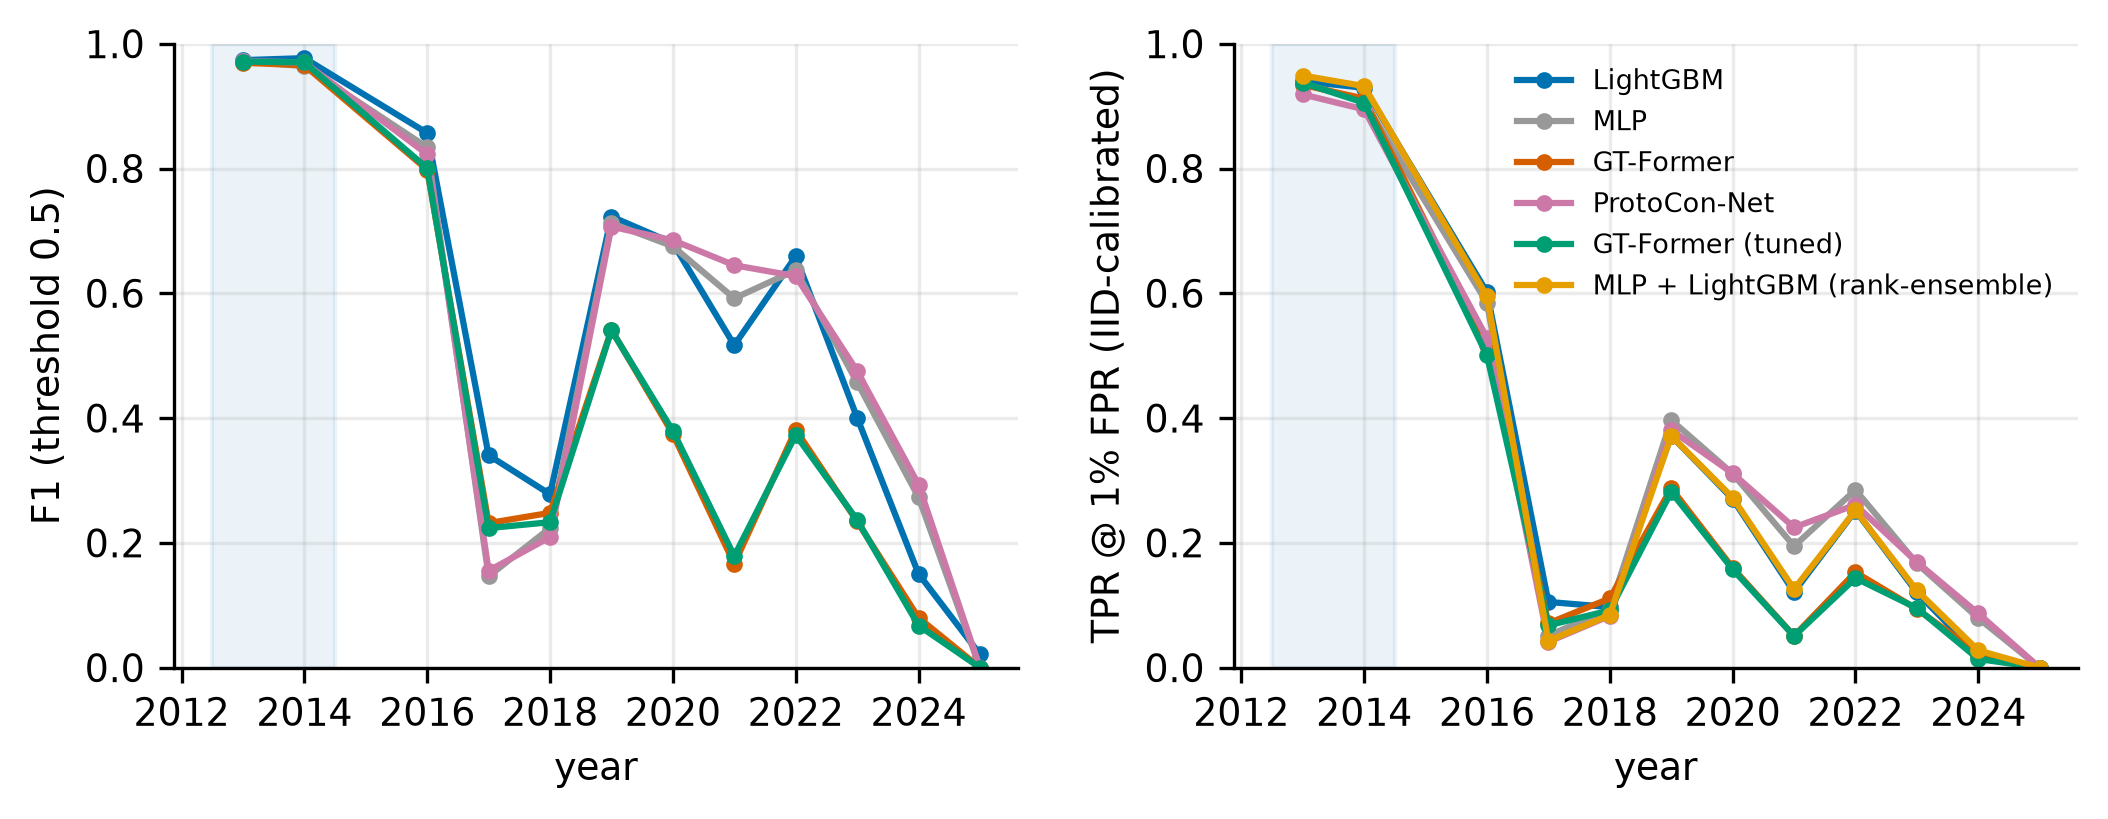
\includegraphics[width=0.9\textwidth]{fig_lamda_drift.png}
\caption{LAMDA: F1 at threshold 0.5 (single models) and TPR at 1\% FPR with the threshold calibrated on the IID benign files, per year; shaded years are the training years.}
\label{fig:lamda-drift}
\end{figure}

\begin{figure}[!htbp]
\centering
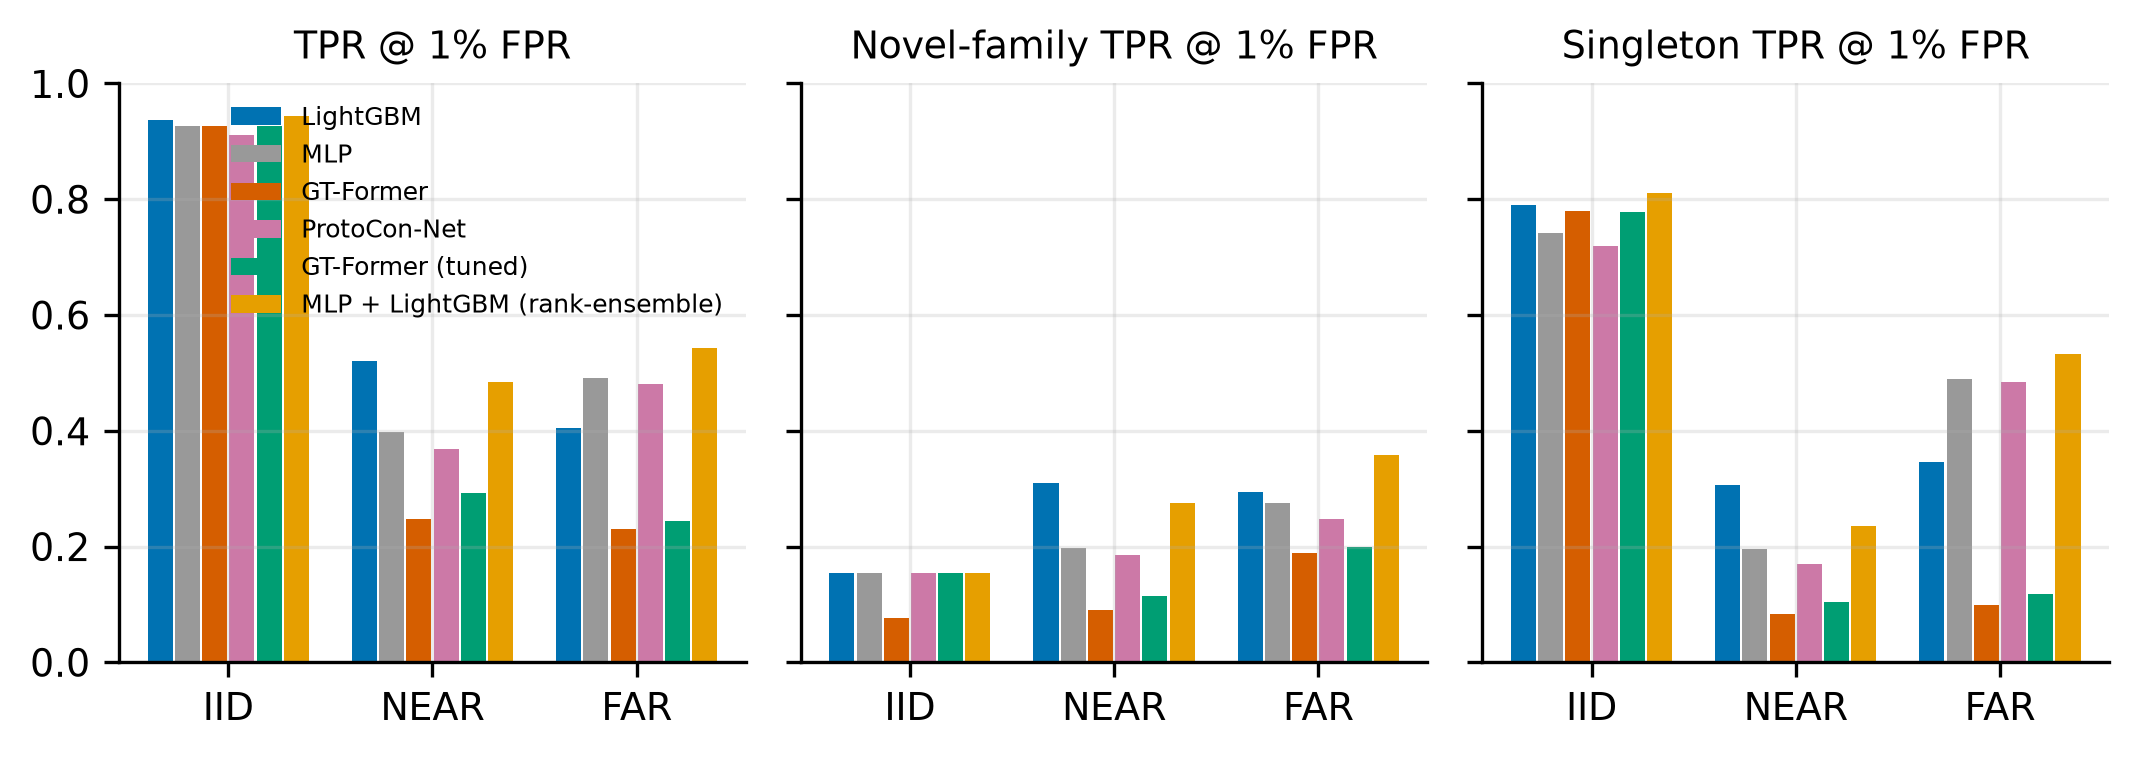
\includegraphics[width=0.85\textwidth]{fig_lamda_regions.png}
\caption{LAMDA: TPR, novel-family TPR and singleton TPR at 1\% FPR per temporal region.}
\label{fig:lamda-regions}
\end{figure}

\subsubsection{Hybrid rank fusion under strong drift}
\label{sec:lamda-fusion}
A rank average of the MLP and \lgbm{} is the best model on the FAR region on every metric: TPR at 1\% FPR 54.4\% versus 40.5\% for \lgbm{} ($+13.8$ points, CI $+13.7$ to $+14.0$), novel-family TPR 35.9\% versus 29.5\% ($+6.4$, CI $+5.9$ to $+6.9$), singleton TPR 53.3\% versus 34.6\% ($+18.7$, CI $+18.4$ to $+18.9$), low-consensus TPR 40.4\% versus 26.3\%, and TPR at 0.1\% FPR 21.1\% versus 12.9\%. On NEAR the ensemble is slightly below \lgbm{} (48.4\% versus 52.1\%, $-3.7$ points) and on IID slightly above (94.4\% versus 93.6\%). Adding the tuned \gtf{} to the ensemble reduces the FAR gain to $+7.3$ points (47.8\% TPR), and a tuned-\gtf{}/\lgbm{} pair is below \lgbm{} (37.4\%): on Drebin features the transformer adds noise, not signal. Figures~\ref{fig:curves-lamda-iid}--\ref{fig:curves-lamda-far} show the confusion matrices and the ROC and precision--recall curves per region at the validation-calibrated threshold, and Table~\ref{tab:cls-lamda} the corresponding classical metrics. The practical recipe is therefore the same on both benchmarks: keep the gradient-boosted benchmark, add one deep model with a different inductive bias, and fuse by rank; the deep partner should be \gtf{} on EMBER version-3 features and a flat MLP on Drebin-style binary features.

\subsubsection{Year-by-year drift}
With the threshold fixed on the IID benign files (Figure~\ref{fig:lamda-drift}), all models collapse in 2017 (TPR at 1\% FPR below 0.12 for every model, F1 below 0.3), partially recover in 2019--2022, and fall to near zero in 2024--2025 when only 635 and 18 malware samples remain in the year. The MLP and ProtoCon-Net stay above \lgbm{} from 2019 onward at the IID-calibrated threshold (2020: 0.32--0.36 versus 0.27; 2021: 0.19--0.23 versus 0.12), which is the year-level view of the FAR result. The 2017 collapse coincides with the year in which the malware share of the corpus halves (21.5\% versus 41--51\% before) and the number of families quintuples (7,436 families versus 1,454 in 2013), so it is a family-composition shift rather than a feature-space shift alone.

%% ------------------------------------------------------------------------------------------------
\subsection{BODMAS}
\label{sec:bodmas}

\subsubsection{Detection on a third benchmark with version-2 features}
BODMAS is easier than the other two: with only six months between the end of training and the last test month, every model exceeds 0.999 ROC-AUC (Table~\ref{tab:bodmas}). It is nevertheless useful for two reasons. It uses EMBER \emph{version-2} features (2,381 dimensions, LIEF-based), so it tests whether the group tokenisation of \gtf{} transfers to a different feature layout, and it contains 1,215 test malware from families never seen in training.

\begin{table}[!htbp]
\centering
\scriptsize
\setlength{\tabcolsep}{2.5pt}
\caption{BODMAS test set (April--September 2020; 60,309 files, 27,701 malware). The tuned \gtf{} is reported as mean $\pm$ standard deviation over five seeds; ensembles use seed 0. Nov.\ = novel-family TPR. Best value per column in bold.}
\label{tab:bodmas}
\begin{tabular}{lccccc}
\toprule
Model & ROC-AUC & \tprat{1} & \tprat{0.1} & Nov.@1\% & Nov.@0.1\% \\
\midrule
\lgbm{} (benchmark config.) & 0.9999 & 0.9985 & 0.9892 & 0.9877 & 0.9465 \\
MLP & 0.9994 & 0.9864 & 0.9652 & 0.9621 & 0.9193 \\
ProtoCon-Net & 0.9993 & 0.9939 & 0.9823 & 0.9638 & 0.9374 \\
\gtf{} (default) & 0.9993 & 0.9884 & 0.9770 & 0.9663 & 0.9440 \\
\gtf{} (tuned), five seeds & $0.9996 \pm 0.0003$ & $0.9954 \pm 0.0014$ & $0.9872 \pm 0.0008$ & $0.9781 \pm 0.0076$ & 0.9572 (seed 0) \\
Fusion: tuned \gtf{} + \lgbm{} & \textbf{0.9999} & \textbf{0.9985} & \textbf{0.9945} & 0.9852 & \textbf{0.9712} \\
Fusion: MLP + \lgbm{} & 0.9999 & 0.9981 & 0.9894 & \textbf{0.9918} & 0.9514 \\
\bottomrule
\end{tabular}
\end{table}

\begin{table}[!htbp]
\centering
\scriptsize
\setlength{\tabcolsep}{2.5pt}
\caption{BODMAS classical metrics at the validation-calibrated 1\% FPR threshold (test set April--September 2020). Fusion = rank fusion of the tuned \gtf{} and \lgbm{}.}
\label{tab:cls-bodmas}
\begin{tabular}{lcccccccccc}
\toprule
Model & Acc. & Bal.\ acc. & Prec. & Recall & Spec. & FPR & F1 & MCC & ROC-AUC & PR-AUC \\
\midrule
\lgbm{} & 0.9963 & 0.9962 & 0.9957 & 0.9961 & 0.9964 & 0.0036 & 0.9959 & 0.9925 & 0.9999 & 0.9999 \\
MLP & 0.9886 & 0.9885 & 0.9876 & 0.9875 & 0.9895 & 0.0105 & 0.9875 & 0.9770 & 0.9994 & 0.9993 \\
\gtf{} (tuned) & 0.9954 & 0.9952 & 0.9970 & 0.9929 & 0.9975 & 0.0025 & 0.9950 & 0.9907 & 0.9998 & 0.9997 \\
Fusion & 0.9971 & 0.9970 & 0.9980 & 0.9957 & 0.9983 & 0.0017 & 0.9968 & 0.9942 & 0.9999 & 0.9999 \\
\bottomrule
\end{tabular}
\end{table}

\curvefigtwo{fig_confusion_BODMAS.png}{fig_roc_pr_BODMAS.png}{BODMAS test set (April--September 2020)}{fig:curves-bodmas}

\subsubsection{Tuning, fusion and monthly drift}
\label{sec:bodmas-findings}
Optuna tuning is worth 0.7 points of TPR at 1\% FPR and 1.0 point at 0.1\% FPR for \gtf{} (98.84\% to $99.54 \pm 0.14$\%; 97.70\% to $98.72 \pm 0.08$\%), and 1.2 points on novel families. The tuned transformer alone is still 0.3 points below \lgbm{} at 1\% FPR (CI $-0.23$ to $-0.12$) and 1.2 points below on novel families, but the rank fusion of the two matches \lgbm{} exactly at 1\% FPR (99.85\%, CI $-0.05$ to $+0.04$) and is better at the strict 0.1\% operating point (99.45\% versus 98.92\%) and on novel families at 0.1\% FPR (97.12\% versus 94.65\%), which is the same complementarity as on EMBER2024. Month by month (Figure~\ref{fig:bodmas-drift}), all models stay above 99\% TPR at the March-calibrated threshold until September 2020, where the tree model dips to 98.4\% and the fusion to 98.9\%; novel-family detection is the only quantity that moves appreciably (94--99\% by month). Figure~\ref{fig:curves-bodmas} shows the confusion matrices and curves at the March-calibrated threshold and Table~\ref{tab:cls-bodmas} the classical metrics. BODMAS therefore confirms that the tokenisation of \gtf{} transfers to the version-2 layout and that the deep/tree fusion is the safest default, while adding little discriminative pressure because the benchmark is close to saturation.

\begin{figure}[!htbp]
\centering
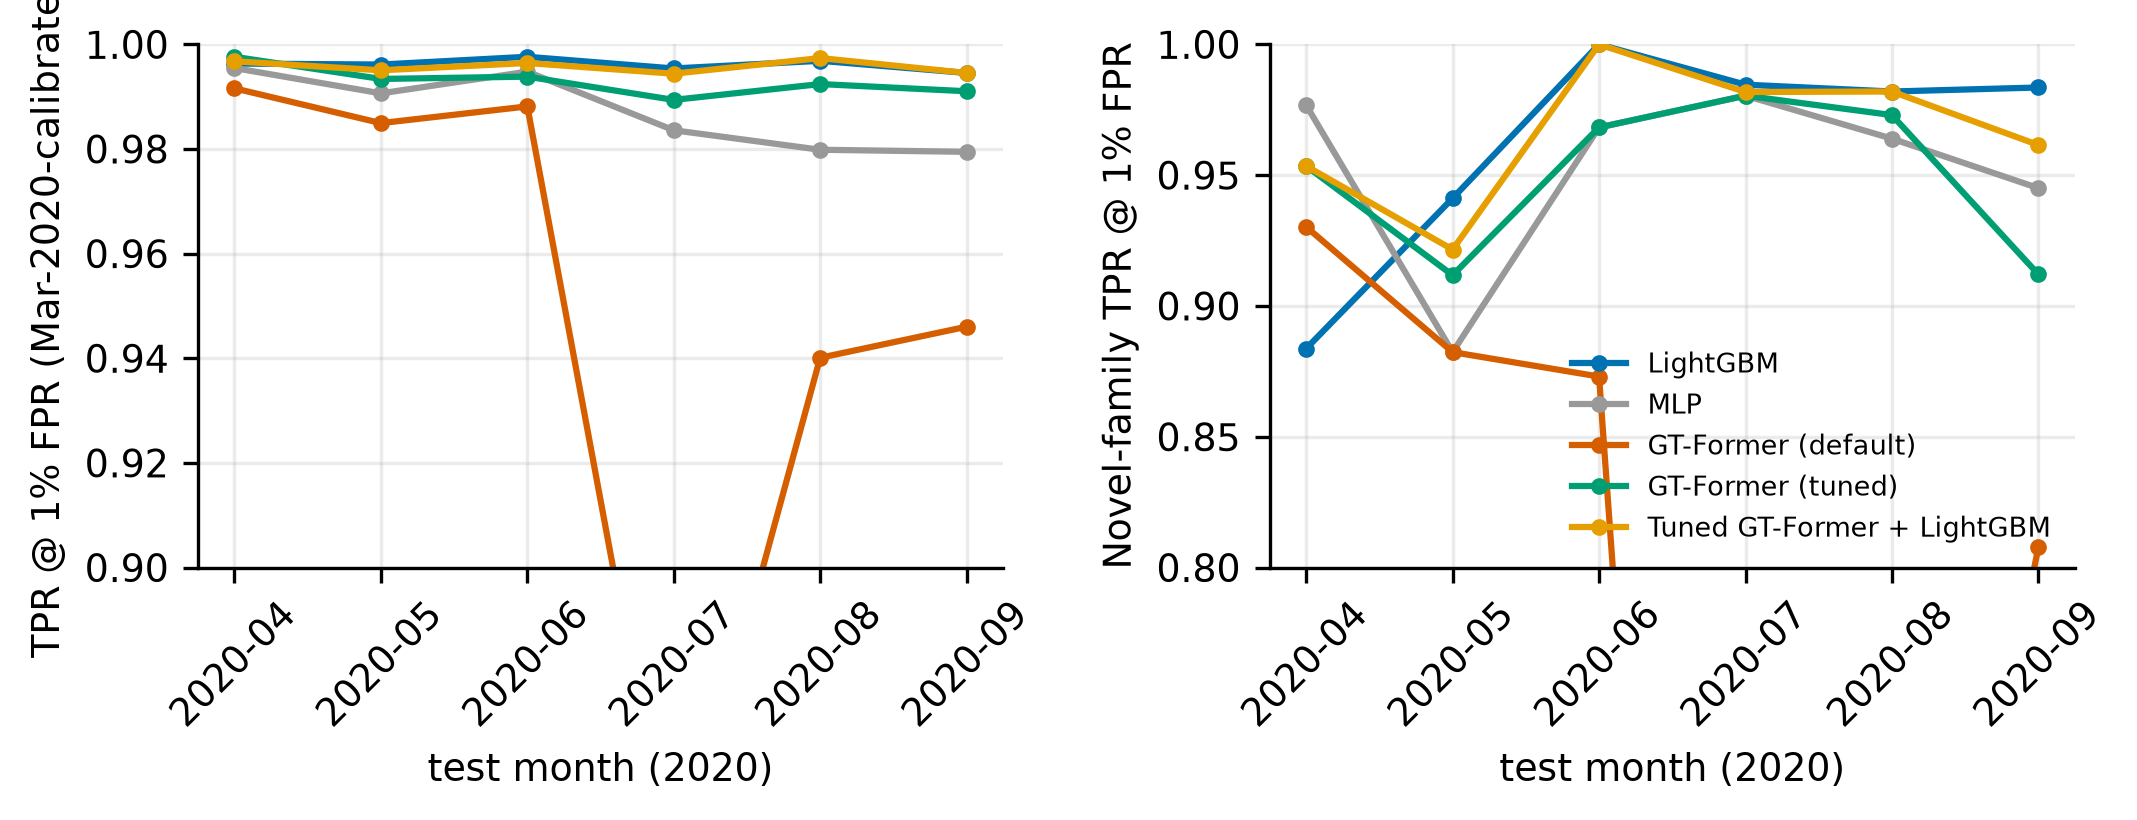
\includegraphics[width=0.9\textwidth]{fig_bodmas_drift.png}
\caption{BODMAS: TPR and novel-family TPR at 1\% FPR per test month (threshold calibrated on March 2020 benign files).}
\label{fig:bodmas-drift}
\end{figure}

%% ------------------------------------------------------------------------------------------------
\section{Explainability: what separates evasive from ordinary malware}
\label{sec:xai}

We explain the two strongest EMBER2024 models with complementary tools: SHAP TreeExplainer values on the \lgbm{} benchmark (3,000 test benign and 3,000 test malware files per format plus every challenge file of that format; Figures~\ref{fig:shap-groups} and \ref{fig:shap-flip} and the last-layer CLS attention of \gtf{} over the twelve group tokens (Figure~\ref{fig:attention}).

\paragraph{Group-level attribution (SHAP)}
On Win32 the benchmark spreads its attribution over the header (16--20\%), sections (10--17\%), imports (13--16\%), strings (12\%) and byte-histogram (11--13\%) groups. Two shifts distinguish challenge files from ordinary malware: attribution to the \emph{imports} group rises from 12.8\% to 15.8\% and to the byte-entropy group from 6.9\% to 8.6\%, while the \emph{pefile warnings} group falls from 8.3\% to 5.3\% and \emph{sections} from 16.5\% to 12.9\%. On Win64 the same pattern appears (imports 14.2\% to 18.1\%, sections 12.1\% to 8.9\%). For the non-PE formats the model can only use the format-agnostic groups (histogram, byte-entropy, strings) and the attribution profile of challenge files is indistinguishable from ordinary malware, which is consistent with their low challenge-set detection.

\paragraph{Feature-level attribution and the direction of the evidence}
The single most important \lgbm{} feature on Win32 and Win64 is the pefile warning ``Suspicious flags set for section'' (mean $|\mathrm{SHAP}|$ 1.26 on Win32 malware). For ordinary malware it pushes \emph{towards} malicious (mean SHAP $+0.56$); for challenge files its mean contribution is \emph{negative} ($-0.72$): evasive files are, on average, well-formed PEs that do not trigger the warning, and the model reads the absence of the warning as evidence of benignness. The same sign flip occurs for the Authenticode features (latest signing time and certificate-chain depth: $+0.29$ on ordinary malware, $-0.10$ and $-0.27$ on challenge files), so a sizeable fraction of evasive malware is signed, and for the \texttt{DLL} image characteristic the positive contribution shrinks from $+0.64$ to $+0.48$ (Figure~\ref{fig:shap-flip}). The benchmark's strongest evidence is \emph{structural sloppiness} (suspicious section flags, missing signatures, unusual checksums and linker versions), and evasive malware is precisely the malware that avoids it.

\begin{figure}[!htbp]
\centering
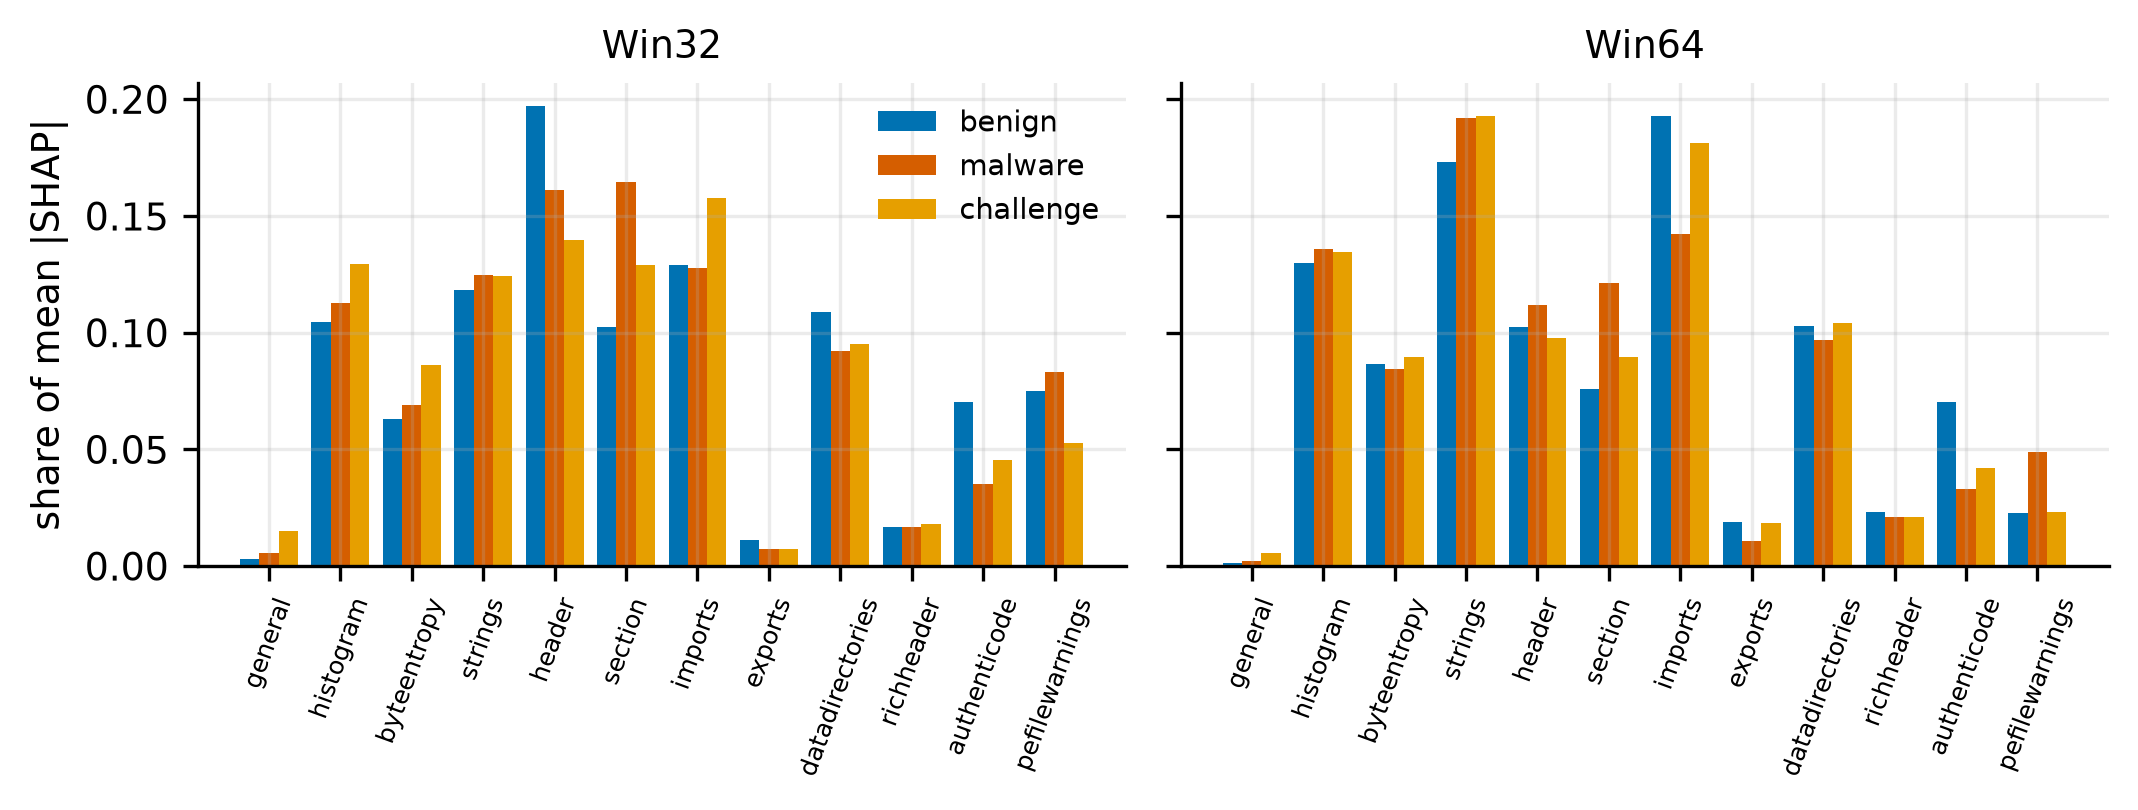
\includegraphics[width=0.9\textwidth]{fig_shap_groups.png}
\caption{\lgbm{} SHAP attribution share per feature group on Win32 and Win64 for benign files, ordinary malware and challenge files.}
\label{fig:shap-groups}
\end{figure}

\begin{figure}[!htbp]
\centering
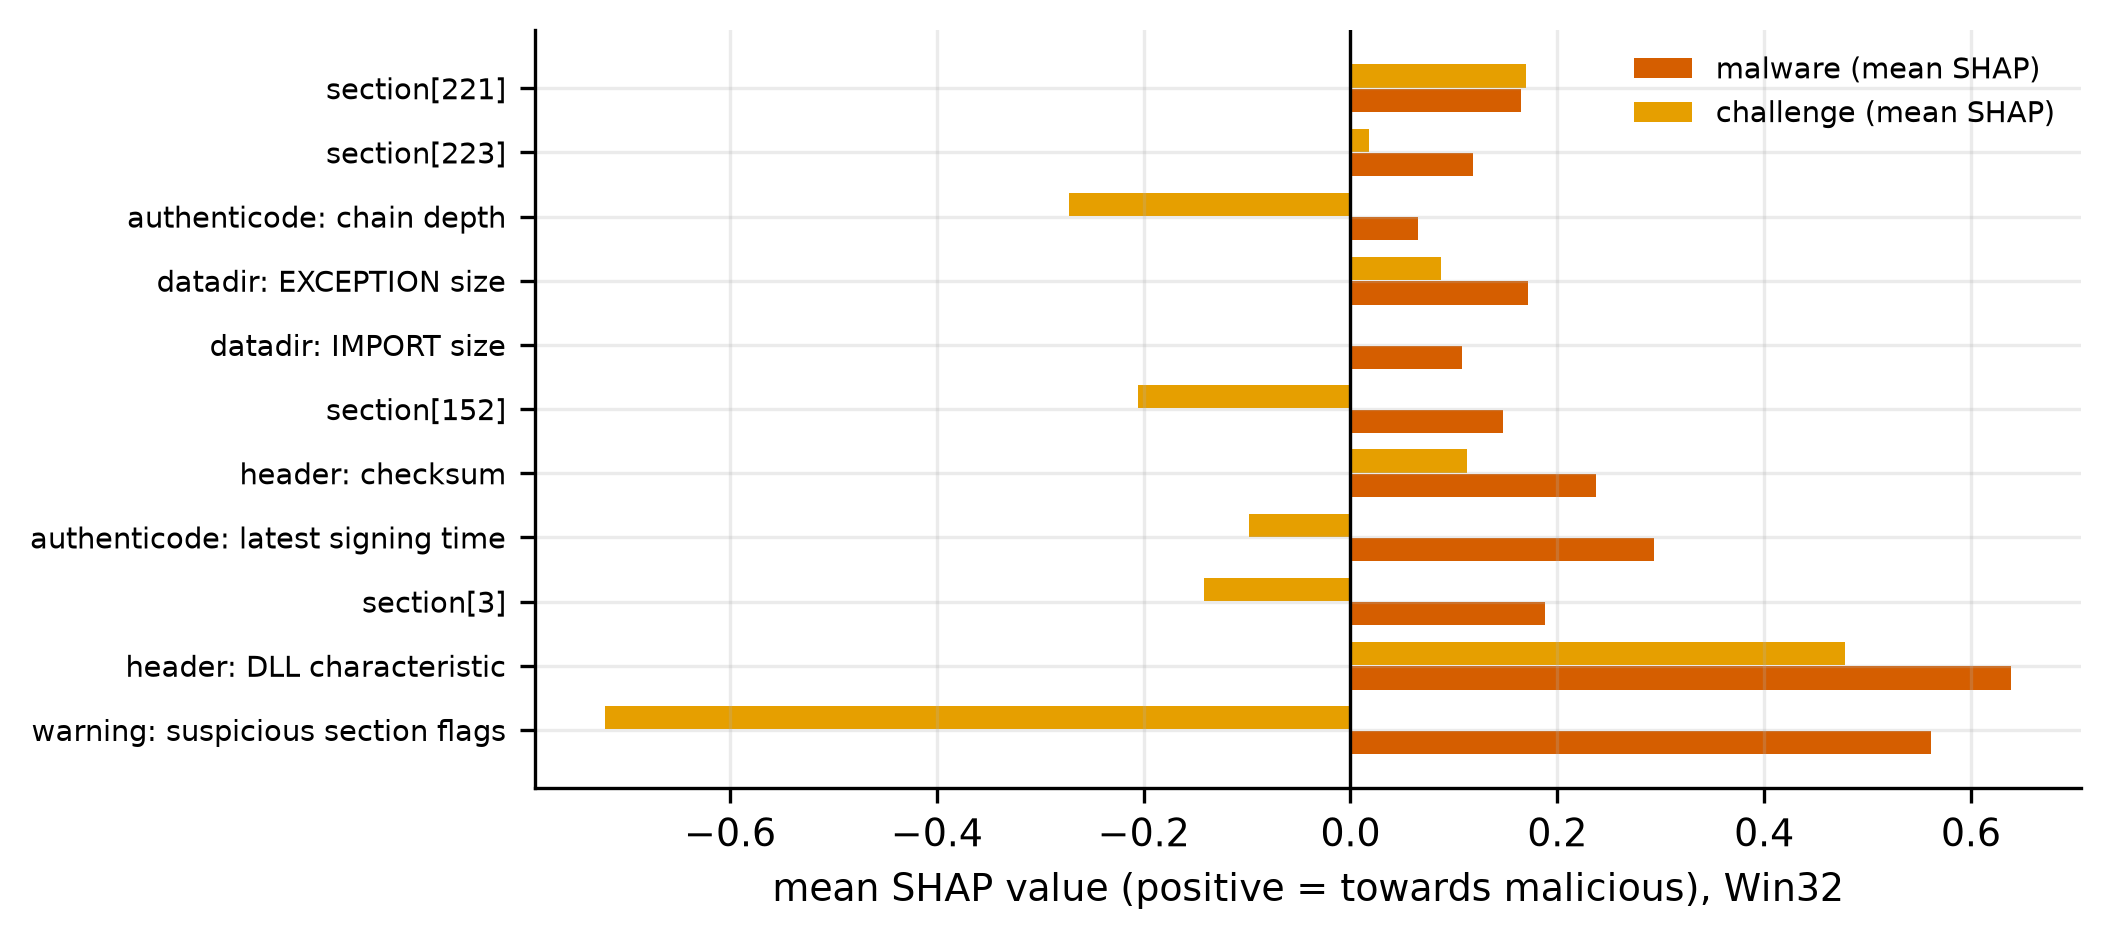
\includegraphics[width=0.8\textwidth]{fig_shap_signflip_win32.png}
\caption{Sign flip of the most important \lgbm{} features between ordinary and challenge malware (Win32, mean SHAP value).}
\label{fig:shap-flip}
\end{figure}

\paragraph{Attention of \gtf{}}
For Win32 benign files the CLS token attends almost uniformly to the twelve groups (0.056--0.094 per token). For ordinary malware it concentrates on imports (0.101) and exports (0.105). For challenge files attention on the exports token doubles (0.215) and attention on strings (0.121) and the rich header (0.098) rises, while attention on the byte histogram (0.039) and general features (0.036) falls (Figure~\ref{fig:attention}). \gtf{} therefore looks for evasive malware in \emph{what the binary exposes} (export table, embedded strings, toolchain fingerprint) rather than in byte statistics, which is a plausible reason why its errors are complementary to the tree model's and why the rank ensemble recovers evasive files at a fixed false-positive budget. On ELF the general token (file size, entropy, is\_pe) receives 25\% of the malware attention, and on PDF the byte histogram dominates for both ordinary and challenge malware.

\begin{figure}[!htbp]
\centering
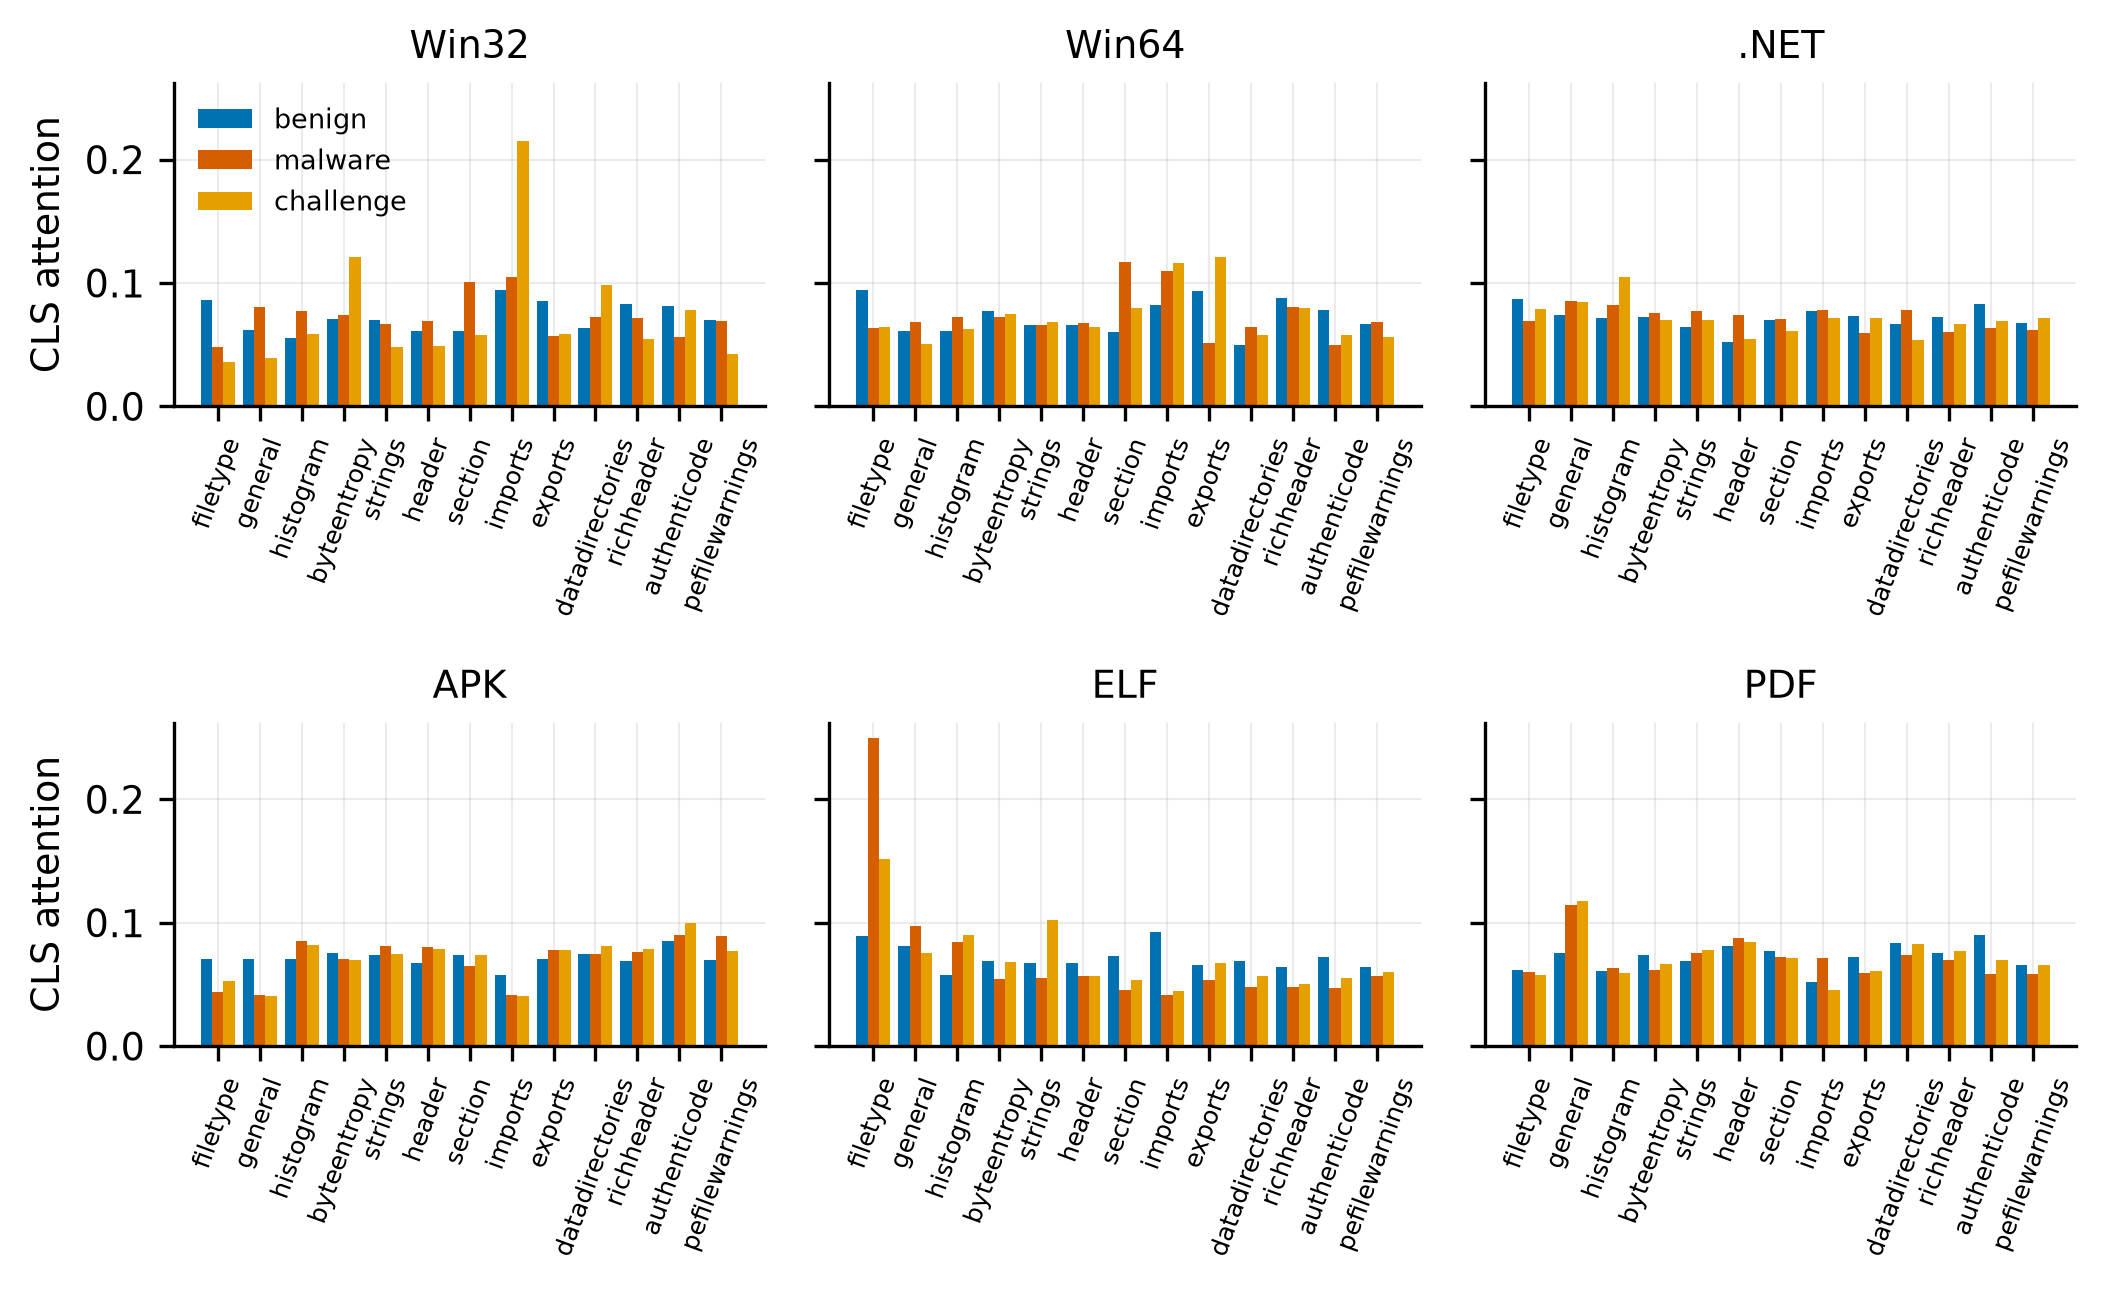
\includegraphics[width=0.9\textwidth]{fig_attention_groups.png}
\caption{\gtf{} last-layer CLS attention over the twelve group tokens for benign files, ordinary malware and challenge files.}
\label{fig:attention}
\end{figure}

\paragraph{Mixture-of-experts routing}
The FR-MoE gate learns format-specific mixtures (Win64: 37\% expert 4 and 25\% expert 3; APK: 24\% expert 5 and 22\% expert 2; .NET: 36\% expert 4), confirming that the file-type signal is used, but no expert specialises exclusively on one format, which matches the finding that FR-MoE gives no accuracy advantage over the flat MLP.

%% ------------------------------------------------------------------------------------------------
\section{Discussion}
\label{sec:discussion}

\paragraph{Why gradient boosting still wins alone in distribution}
EMBER version-3 and Drebin features are heavy-tailed counts, hashed bins and binary indicators on which axis-aligned splits are a near-perfect inductive bias; the deep models need 8--12 epochs to reach 0.9975 AUC where \lgbm{} reaches 0.9982, and their deficit is concentrated at strict FPR, where a handful of high-scoring benign files matter.

\paragraph{Why fusion helps where it matters}
The deep model's errors are partly independent of the tree model's, since Section~\ref{sec:xai} shows that the two use different evidence; averaging ranks recovers evasive and drifted files that the tree ranks below the operating threshold. The gain is largest exactly where single models are weakest: the challenge set on EMBER2024 and the far-future, singleton-heavy years of LAMDA ($+13.8$ and $+18.7$ points).

\paragraph{Why the deep model's robustness to drift differs between benchmarks}
On LAMDA the MLP degrades more gracefully than \lgbm{} over 2018--2025, while on the twelve EMBER2024 test weeks the tree model is at least as stable. The FAR region of LAMDA is dominated by singletons (131,648 of 213,274 malware) and by a benign-heavy class balance; a smooth, high-capacity decision function generalises to these better than sharp thresholds tuned on 2013--2014. The twelve EMBER2024 test weeks contain too little drift to show the same effect.

\paragraph{Why consensus and family objectives failed}
Challenge files are low-consensus \emph{at their final rescan}, but the training-time consensus of ordinary malware is only weakly related to how a \emph{different} file evades; CAM therefore reshapes the boundary for the wrong files. Family-adversarial training removes discriminative information: it lowers strict-FPR TPR on both benchmarks and does not help novel families or singletons. A more promising direction is to use consensus for \emph{sample selection} (curriculum or hard-example mining) and family labels for \emph{evaluation}, not for invariance.

\paragraph{Benchmark hygiene}
Every paper that trained on the raw EMBER2024 Hugging Face files trained on each record twice. This creates no train/test leakage, but it doubles reported dataset sizes and epoch costs and changes early-stopping behaviour. We release the SHA-256 keep-masks and the exact LAMDA split indices.

\paragraph{Limitations}
The study uses static features only and three benchmarks, one of which (BODMAS) is near saturation. Antivirus consensus is a noisy proxy for evasiveness, and the ClarAVy and AVClass2 confidences were not exploited. We did not evaluate functionality-preserving adversarial attacks. The deep models were trained for a fixed short budget on one GPU, and although Optuna tuning narrowed the gap to \lgbm{} it did not close it. The smallest EMBER formats (ELF and PDF) and \gtf{} on LAMDA give seed-unstable results, and the 2024--2025 years of LAMDA contain too few malware samples for reliable TPR estimates.

%% ------------------------------------------------------------------------------------------------
\section{Conclusion}
\label{sec:conclusion}

Under an operational lens the picture on EMBER2024, LAMDA and BODMAS is consistent. The gradient-boosted benchmark is still the best single model in distribution; the deep architectures we propose come close (Optuna tuning brings \gtf{} within 1.5 points of \lgbm{} at 0.1\% FPR on Win32 and within 0.3 points at 1\% FPR on BODMAS) but do not overtake it; the consensus- and family-aware objectives we designed are harmful; and a rank fusion of the benchmark with one deep model of a different inductive bias is the best detector we found for evasive malware, novel families and far-future drift, with statistically significant gains on all three benchmarks. Explainability shows that the benchmark's evidence for maliciousness is structural sloppiness that evasive malware avoids, and that the transformer looks elsewhere (export tables, strings, toolchain fingerprints), which is why the two are complementary. We release the protocol, the hygiene fixes and every score file so that future work can be compared at the same operating points.

\section*{Data Availability}
The three benchmarks are publicly available from their authors.
\begin{itemize}[leftmargin=*]
    \item \textbf{EMBER2024} (Apache-2.0): \url{https://huggingface.co/datasets/joyce8/EMBER2024}
    \item \textbf{LAMDA} (MIT): \url{https://huggingface.co/datasets/IQSeC-Lab/LAMDA}
    \item \textbf{BODMAS}: \url{https://whyisyoung.github.io/BODMAS/}
\end{itemize}
The code of this paper (feature vectorisation, de-duplication masks, the exact LAMDA and BODMAS split indices, the \lgbm{} variants, the \gtf{}, FR-MoE and ProtoCon-Net implementations, Optuna tuning, rank fusion, bootstrap tests, tables, figures and the SHAP and attention analyses), all trained models and all score files for random seeds 0--4 are released at \url{https://github.com/kmkholm/GTFormer} (score files and trained models are attached to the repository release).

\bibliography{refs}

\section*{Author Contributions}
\textbf{Mohammed Tawfik}: Conceptualization, Methodology, Software, Formal Analysis, Investigation, Writing -- Original Draft.
\textbf{Belal Al-sellami}: Methodology, Data Curation, Validation, Writing -- Review \& Editing, Corresponding Author.
\textbf{Mohamed Heshmat}: Investigation, Formal Analysis, Visualization, Writing -- Review \& Editing.
\textbf{Islam S.~Fathi}: Validation, Resources, Writing -- Review \& Editing.
\textbf{Warda M.~Shaban}: Supervision, Project Administration, Writing -- Review \& Editing.
All authors reviewed and approved the final manuscript. [Roles to be confirmed by the authors.]

\section*{Declarations}
\subsection*{Funding}
This research received no specific grant from any funding agency in the public, commercial, or not-for-profit sectors.

\subsection*{Ethics Declaration}
Not applicable.

\subsection*{Competing Interests}
The authors declare no competing interests.

\end{document}
